\section{Parallelizzazione}
\label{sec:parallelizzazione}
\subsection{Frazione parallelizzabile e scelte di decomposizione}

La frazione parallelizzabile $P$ non misura una proporzione di righe di codice,
bensì la quota del tempo seriale $T_1$ spesa nella parte parallelizzabile.
Individuarla richiede di distinguere, nel programma seriale, ciò che costituisce
lavoro indipendente da ciò che resta intrinsecamente seriale.

L'unità naturale di parallelismo è il pixel: il kernel della
sezione~\ref{sec:seriale-codice} lo elabora in tre passi, tutti indipendenti
dagli altri pixel.
\begin{enumerate}
  \item \textbf{Calcolo del punto $c$.} La conversione dell'indice
  $(\text{row}, \text{col})$ nel punto del piano complesso usa soltanto variabili
  locali, senza dipendenze da altri pixel.
  \item \textbf{Calcolo dell'escape time.} La ricorrenza è sequenziale
  \emph{dentro} il pixel, perché l'iterazione $n+1$ dipende dalla $n$, ma ogni
  pixel la esegue in autonomia: il parallelismo risiede \emph{fra} i pixel. È la
  parte in cui si concentra la quasi totalità del tempo, e quella in cui la
  variabilità del numero di iterazioni si traduce in sbilanciamento del carico.
  \item \textbf{Scrittura del risultato.} L'assegnamento
  \verb|data[row * width + col]| usa un indice univoco per ogni pixel: non vi
  sono conflitti di scrittura, e la memoria condivisa non richiede né mutua
  esclusione né sincronizzazione.
\end{enumerate}

Resta fuori dal task la sola frazione seriale: l'allocazione della matrice,
l'inizializzazione e la gestione delle strutture dati. Il suo costo è stimato in
circa un decimo di millisecondo su $722$~ms (sezione~\ref{sec:serial-time}),
cioè $1 - P \approx 10^{-4}$: a $p = 32$ la legge di Amdahl limita lo speedup a
circa $31{,}9$, al di sopra di ogni valore misurato. Le perdite di efficienza
osservate nelle sezioni seguenti vanno dunque cercate altrove, nella
distribuzione del lavoro.

Quanto alla decomposizione, i due paradigmi CPU non distribuiscono singoli pixel
ma righe intere, per le ragioni discusse nella sezione~\ref{sec:openmp}; la GPU,
che dispone di migliaia di thread, assegna invece a ciascuno un solo pixel
(sezione~\ref{sec:cuda}).

%---------------PREVISIONI DAL SERIALE-----------------
% Collocata prima di OpenMP e MPI, e non nel capitolo seriale: le analisi dei
% due paradigmi usano lambda_p per spiegare i propri risultati, e le regole vanno
% lette accanto ai meccanismi che le realizzano. I valori dipendono dal solo
% profilo {w_r} del baseline (data/block_imbalance.csv).
\subsection{Previsioni dal profilo di carico seriale}
\label{sec:serial-pred-lambdaP}

Applicando al profilo $\{w_r\}$ misurato nella sezione~\ref{serial_results} le
tre regole di assegnamento definite nella sezione~\ref{sec:serial-predizione}, si
ottengono lo sbilanciamento effettivo $\lambda_p = p\,M(p)/\mathcal{W}$ e il
limite $S(p) \le p/\lambda_p$ di ciascuna decomposizione, prima ancora che il
codice parallelo esista.

Le previsioni non sono formulate per implementazione, ma per regola di
assegnamento: ciascuna regola è realizzata, con meccanismi diversi, da più di un
paradigma (tabella~\ref{tab:regole-paradigmi}), e la stessa riga di previsione va
perciò confrontata con le misure di entrambi. La versione CUDA resta fuori da
questo quadro: operando a granularità di pixel, non è descritta dal profilo di
riga, e il suo predittore, ricavato dalla stessa matrice degli escape time, è
presentato nella sezione~\ref{sec:cuda-previsioni}.
\vspace{2,5mm}
\begin{table}[htbp]
    \centering
    \begin{tabular}{lll}
        \hline
        Regola & OpenMP & MPI \\
        \hline
        blocchi  & \texttt{schedule(static)} & decomposizione \texttt{block} \\
        ciclica  & --- (non misurata) & decomposizione \texttt{cyclic} \\
        dinamica & \texttt{schedule(dynamic,1)} & master--worker \\
        \hline
    \end{tabular}
    \caption{Corrispondenza fra le tre regole di assegnamento predette dal profilo
    di carico seriale e i meccanismi che le realizzano nei due paradigmi CPU. La
    regola ciclica è esercitata dal solo MPI: lo sweep OpenMP non include
    \texttt{schedule(static,1)}, che ne sarebbe l'equivalente a memoria condivisa.}
    \label{tab:regole-paradigmi}
\end{table}
\vspace{2,5mm}
\begin{table}[H]
    \centering
    \begin{tabular}{ccccccc}
        \hline
        & \multicolumn{2}{c}{\textbf{blocchi}} & \multicolumn{2}{c}{\textbf{ciclica}} & \multicolumn{2}{c}{\textbf{dinamica}} \\
        \textbf{p} & $\lambda_p$ & $S \le$ & $\lambda_p$ & $S \le$ & $\lambda_p$ & $S \le$ \\ \hline
        2  & 1{,}0000 & 2{,}00  & 1{,}0000 & 2{,}00  & 1{,}0000 & 2{,}00 \\
        4  & 1{,}8798 & 2{,}13  & 1{,}0001 & 4{,}00  & 1{,}0000 & 4{,}00 \\
        8  & 2{,}3489 & 3{,}41  & 1{,}0011 & 7{,}99  & 1{,}0000 & 8{,}00 \\
        16 & 2{,}5937 & 6{,}17  & 1{,}0017 & 15{,}97 & 1{,}0000 & 16{,}00 \\
        32 & 2{,}6619 & 12{,}02 & 1{,}0095 & 31{,}70 & 1{,}0000 & 32{,}00 \\
    \end{tabular}
    \caption{Sbilanciamento effettivo $\lambda_p$ e limite superiore allo
    speedup $S \le p/\lambda_p$, calcolati dal solo profilo di carico
    seriale ($1024\times1024$, $N_{\max}=1000$) per le tre regole di
    assegnamento delle righe.}
    \label{tab:serial_pred_lambdaP}
\end{table}

La tabella~\ref{tab:serial_pred_lambdaP} quantifica il costo della scelta
di decomposizione a parità di hardware e di numero di processori.  Con
$32$ unità di calcolo, l'assegnamento a blocchi non può superare uno
speedup di $12{,}02$: il $62\%$ del tempo di calcolo complessivo va perso in
attesa del processore più carico, poiché le righe centrali costose sono contigue e finiscono
tutte nello stesso blocco.  La sola sostituzione dell'assegnamento
contiguo con quello ciclico porta il limite a $31{,}70$, cioè a
un'efficienza teorica del $99\%$: l'interlacciamento distribuisce le
righe pesanti fra tutti i processori.  Si noti anche il caso $p=2$, in
cui tutte e tre le regole danno $\lambda_p = 1$ esattamente.  Per le due
regole statiche il motivo è la simmetria del dominio rispetto all'asse
reale: la riga $r$ e la riga $H{-}1{-}r$ campionano punti coniugati e
hanno perciò carico identico, cosicché sia la partizione in due metà
contigue sia quella fra righe pari e dispari risultano bilanciate in modo
esatto.  Per la regola dinamica il motivo è invece che la riga più
pesante, pari a $2{,}76$ volte la media, resta molto al di sotto della
quota equa $\mathcal{W}/2$.  Con due soli processori, dunque, la scelta
della decomposizione è irrilevante: le differenze fra le strategie
emergono solo quando i blocchi diventano abbastanza piccoli da non
contenere più un campione rappresentativo del profilo.

Si osserva infine la monotonia annunciata in~\eqref{eq:lambdaP}: per
l'assegnamento a blocchi $\lambda_p$ cresce con $p$ ($1{,}00 \to 2{,}66$)
avvicinandosi al valore intrinseco $\lambda = 2{,}76$ misurato nella
sezione~\ref{serial_results}, che
verrebbe raggiunto nel caso limite $p = H$.  Il margine fra $2{,}66$ e
$2{,}76$ misura quanta compensazione fra picchi e valli
sopravvive ancora aggregando $32$ righe per blocco.

%--------------------- OPEN_MP -------------------
\subsection{OpenMP: memoria condivisa}
\label{sec:openmp}

Nel modello a memoria condivisa i thread non si scambiano dati in modo
esplicito: leggono e scrivono la stessa matrice degli escape time,
residente in un unico spazio di indirizzamento. Il grado di parallelismo non è
quindi fissato dal numero di pixel --- che sono milioni --- ma dal numero di
core del nodo: OpenMP istanzia un pool fisso di thread, e le clausole di
schedule non regolano \emph{quanti} thread esistano, bensì la granularità con
cui il lavoro viene ripartito tra essi.

Sebbene nella sezione~\ref{sec:parallelizzazione} si sia individuato nel
singolo pixel l'unità indipendente della computazione, non conviene farne
l'unità di \emph{ripartizione}. Assegnare un pixel per volta a ciascun thread
introduce due costi che si sommano senza aggiungere parallelismo. Primo, un
costo di scheduling: ogni prelievo di una nuova unità richiede un accesso a un
contatore condiviso, e per un'unità da poche centinaia di iterazioni tale costo
non è trascurabile rispetto al calcolo stesso. Secondo, il \emph{false sharing}: pixel
adiacenti sulla stessa riga cadono nella medesima cache line, che rimbalzerebbe
tra i core scriventi.

Si ripartisce quindi il ciclo esterno, sulle righe: a ciascun thread è
assegnato un gruppo di righe intere. Il costo di scheduling viene così
ammortizzato sui pixel della riga, e il false sharing si riduce alle sole righe
di confine fra due gruppi, dove l'ultimo pixel di una riga e il primo della
successiva possono condividere una cache line: un effetto trascurabile.

La decomposizione per righe rende anche immediata la correttezza. Ogni thread
scrive esclusivamente nelle celle delle proprie righe: gli insiemi di celle
scritte sono disgiunti, non esiste alcuna \emph{race condition} sui dati e non
è necessaria alcuna sincronizzazione in scrittura. Il false sharing residuo è
un problema di prestazioni, non di correttezza. La coincidenza del
checksum con quello della baseline seriale è la verifica sperimentale di questa
assenza di race: una sovrapposizione in scrittura altererebbe la matrice e il
checksum non tornerebbe.

% ============================================================
\subsubsection{Design dello sweep}
\label{sec:openmp-sweep}
% ============================================================

La domanda progettuale non è quanto parallelizzare, ma \emph{con quale regola
assegnare le righe ai thread}. La risposta non è unica: esistono politiche con
proprietà di bilanciamento e di coordinamento molto diverse, e confrontarle
empiricamente è l'obiettivo dell'esperimento. Lo sweep sistema cinque politiche
sullo stesso intervallo di $p \in \{2, 4, 8, 16, 32\}$ thread, a griglia
$1024^2$ e $N_{\max} = 1000$ fissati: variare le sole leve di scheduling
isola l'effetto della politica da quello del carico e del numero di core.

\paragraph{\texttt{static}.}
Assegna in anticipo a ogni thread un blocco contiguo di $H/p$
righe consecutive. La distribuzione è decisa prima di iniziare: non esiste coda
a runtime, il costo di coordinamento è zero. Il prezzo è che un thread che
esaurisce il proprio blocco resta inattivo fino a che l'ultimo thread non ha
terminato il suo. Poiché le righe che attraversano l'interno dell'insieme
costano fino a $N_{\max}$ iterazioni per pixel mentre quelle ai bordi sfuggono
in poche iterazioni, i blocchi centrali concentrano il lavoro. \texttt{static}
è quindi il caso limite in cui il bilanciamento è interamente delegato alla
geometria del problema: con un profilo di carico uniforme sarebbe ottimale; con
il profilo del Mandelbrot è fortemente sfavorevole. È precisamente questo confronto che motiva la
scelta della politica come primo estremo dello sweep.

\paragraph{\texttt{dynamic} con chunk variabile.}
Invece di assegnare tutto il lavoro in anticipo, il runtime mantiene una coda
di chunk: quando un thread ha esaurito le righe che stava elaborando, preleva il
chunk successivo. Il ribilanciamento è automatico: i thread veloci --- quelli
che hanno elaborato righe leggere --- riprendono subito lavoro, mentre quelli
lenti restano occupati senza lasciare altri in attesa.

La dimensione del chunk governa un compromesso tra due costi opposti. Un chunk
piccolo garantisce un bilanciamento quasi perfetto --- nessun thread può restare
bloccato su un blocco pesante a lungo --- ma moltiplica il numero di accessi
alla coda condivisa, ciascuno dei quali richiede un'operazione di
sincronizzazione interna. Un chunk grande riduce l'overhead di coordinamento,
ma riavvicina il comportamento a quello statico: un thread potrebbe caricarsi di
$k$ righe tutte pesanti e diventare il collo di bottiglia. Per rendere visibile
questo trade-off lo sweep campiona tre valori: $k \in \{1, 16, 64\}$ righe.
\texttt{dynamic,1} è l'estremo di bilanciamento massimo, \texttt{dynamic,64}
quello di overhead minimo; \texttt{dynamic,16} è il punto intermedio. Il chunk
ottimale --- quello che minimizza il tempo complessivo --- emerge dai dati e
costituisce un risultato dell'analisi, non un'ipotesi.

\paragraph{\texttt{guided}.}
È il compromesso adattivo tra i due estremi. Come \texttt{dynamic}, mantiene
una coda; a differenza di esso, la dimensione del chunk non è fissa: parte
proporzionale al lavoro rimasto e si riduce nel tempo. All'inizio, quando ci
sono molte righe disponibili, il chunk è ampio --- l'overhead di coda è basso
come in \texttt{static}. Verso la fine, quando rimangono poche righe e il
rischio è che un thread si trovi con un blocco pesante mentre gli altri sono
fermi, il chunk si rimpicciolisce, replicando la granularità fine di
\texttt{dynamic,1} nel momento in cui conta di più. L'idea è ottenere il
bilanciamento di \texttt{dynamic} pagando una frazione dell'overhead.

% ============================================================
\subsubsection{Metriche specifiche}
\label{sec:openmp-metriche}
% ============================================================

OpenMP non introduce metriche proprie: speedup, efficienza e $e(p)$ restano
quelle comuni della sezione~\ref{sec:metriche-comuni}, calcolate sui soli tempi.
Ciò che è specifico del paradigma è il legame fra la politica di scheduling e lo
sbilanciamento previsto dal profilo seriale. In questo quadro $\mathrm{CoV}$ è
l'indicatore che stabilisce \emph{a priori} se lo scheduling dinamico convenga:
un valore elevato segnala una dispersione del carico tale da giustificarne il
costo di coordinamento, mentre un valore prossimo a zero renderebbe già ottimale
la politica statica.

% ============================================================
\subsubsection{Frammenti di codice rilevanti}
\label{sec:openmp-codice}
% ============================================================

Rispetto al kernel seriale il file OpenMP differisce per due sole righe di
codice, la direttiva sul ciclo esterno e l'etichetta che identifica il paradigma
nel CSV; le funzioni di supporto restano identiche byte per byte, ed è questo a
garantire
la coincidenza del checksum. Qui si commentano solo le scelte rilevanti; il
codice completo è in \repofile{mandelbrot/src/mandelbrot_omp.cpp}.

La differenza sostanziale è una singola direttiva sul ciclo esterno:

\begin{verbatim}
#pragma omp parallel for schedule(runtime)
for (int row = 0; row < computed_rows; ++row) {
    // inner column loop: identical to the serial kernel
    ...
}
\end{verbatim}

Non è necessaria alcuna clausola di data-sharing: le variabili dichiarate nel
corpo del ciclo sono private per costruzione, mentre la matrice è condivisa ma
scritta da ogni thread solo sulle celle delle proprie righe. La scelta
implementativa che conta è \texttt{schedule(runtime)}: la politica non è
fissata nel codice ma letta a esecuzione dalla variabile d'ambiente
\texttt{OMP\_SCHEDULE}, così che un unico binario copra tutte le politiche
variando solo il job script, senza ricompilazione. Il confronto tra politiche è
dunque uno sweep di configurazioni sullo stesso eseguibile, non binari distinti.

Lo sweep è eseguito da un unico job SLURM su un singolo nodo e si ferma a $32$
thread, la capienza di un socket (sezione~\ref{sec:ambiente}). I thread sono
ancorati ai core (\texttt{OMP\_PLACES=cores}, \texttt{OMP\_PROC\_BIND=close}),
così che l'intera campagna resti in un solo dominio NUMA e che la migrazione dei
thread non aggiunga rumore al tempo minimo. Il tempo $T_1$ è misurato nello
stesso job con il binario seriale, e non con la versione OpenMP a un thread, e
tutte le misure usano il kernel \emph{bare}.

% ============================================================
\subsubsection{Analisi dei risultati}
\label{sec:openmp-risultati}
% ============================================================

Il confronto mette a sistema le cinque politiche sullo stesso intervallo di $p$
(da $2$ a $32$ thread), a risoluzione e $N_{\max}$ fissati. La
tabella~\ref{tab:openmp-schedule} raccoglie i $25$ punti misurati, e la
figura~\ref{fig:openmp-schedules} ne riporta gli speedup.
\vspace{2,5mm}
\begin{table}[htbp]
    \centering
    \begin{tabular}{lrrrrr}
        \hline
        Politica & $p$ & $T_\parallel(p)$ [s] & $S(p)$ & $E(p)$ & $e(p)$ \\
        \hline
        seriale & 1 & $0{,}72563$ & --- & --- & --- \\
        \hline
        \texttt{static} & 2  & $0{,}36076$ & $2{,}011$  & $1{,}006$ & $-0{,}0056$ \\
        \texttt{static} & 4  & $0{,}34035$ & $2{,}132$  & $0{,}533$ & $0{,}2921$ \\
        \texttt{static} & 8  & $0{,}21280$ & $3{,}410$  & $0{,}426$ & $0{,}1923$ \\
        \texttt{static} & 16 & $0{,}11748$ & $6{,}176$  & $0{,}386$ & $0{,}1060$ \\
        \texttt{static} & 32 & $0{,}06048$ & $11{,}999$ & $0{,}375$ & $0{,}0538$ \\
        \hline
        \texttt{dynamic,1} & 2  & $0{,}36079$ & $2{,}011$  & $1{,}006$ & $-0{,}0056$ \\
        \texttt{dynamic,1} & 4  & $0{,}18043$ & $4{,}022$  & $1{,}005$ & $-0{,}0018$ \\
        \texttt{dynamic,1} & 8  & $0{,}09028$ & $8{,}037$  & $1{,}005$ & $-0{,}0007$ \\
        \texttt{dynamic,1} & 16 & $0{,}04542$ & $15{,}977$ & $0{,}999$ & $0{,}0001$ \\
        \texttt{dynamic,1} & 32 & $0{,}02342$ & $30{,}988$ & $0{,}968$ & $0{,}0011$ \\
        \hline
        \texttt{dynamic,16} & 2  & $0{,}36091$ & $2{,}011$  & $1{,}005$ & $-0{,}0053$ \\
        \texttt{dynamic,16} & 4  & $0{,}18041$ & $4{,}022$  & $1{,}006$ & $-0{,}0018$ \\
        \texttt{dynamic,16} & 8  & $0{,}09132$ & $7{,}946$  & $0{,}993$ & $0{,}0010$ \\
        \texttt{dynamic,16} & 16 & $0{,}04821$ & $15{,}050$ & $0{,}941$ & $0{,}0042$ \\
        \texttt{dynamic,16} & 32 & $0{,}03126$ & $23{,}211$ & $0{,}725$ & $0{,}0122$ \\
        \hline
        \texttt{dynamic,64} & 2  & $0{,}36073$ & $2{,}012$  & $1{,}006$ & $-0{,}0057$ \\
        \texttt{dynamic,64} & 4  & $0{,}18678$ & $3{,}885$  & $0{,}971$ & $0{,}0099$ \\
        \texttt{dynamic,64} & 8  & $0{,}11765$ & $6{,}168$  & $0{,}771$ & $0{,}0424$ \\
        \texttt{dynamic,64} & 16 & $0{,}11746$ & $6{,}178$  & $0{,}386$ & $0{,}1060$ \\
        \texttt{dynamic,64} & 32 & $0{,}11767$ & $6{,}167$  & $0{,}193$ & $0{,}1351$ \\
        \hline
        \texttt{guided} & 2  & $0{,}36056$ & $2{,}012$  & $1{,}006$ & $-0{,}0062$ \\
        \texttt{guided} & 4  & $0{,}26171$ & $2{,}773$  & $0{,}693$ & $0{,}1475$ \\
        \texttt{guided} & 8  & $0{,}13250$ & $5{,}477$  & $0{,}685$ & $0{,}0658$ \\
        \texttt{guided} & 16 & $0{,}06511$ & $11{,}144$ & $0{,}697$ & $0{,}0290$ \\
        \texttt{guided} & 32 & $0{,}03315$ & $21{,}892$ & $0{,}684$ & $0{,}0149$ \\
        \hline
    \end{tabular}
    \caption{OpenMP: tempo, speedup, efficienza e frazione seriale sperimentale per
    ogni combinazione (politica, chunk, thread). Griglia $1024^2$, $N_{\max}=1000$,
        kernel \emph{bare}, un socket di un unico nodo, minimo su $R=5$ ripetizioni.
        Tutte le righe condividono lo stesso checksum della baseline seriale.}
    \label{tab:openmp-schedule}
\end{table}
\begin{figure}[htbp]
    \centering
    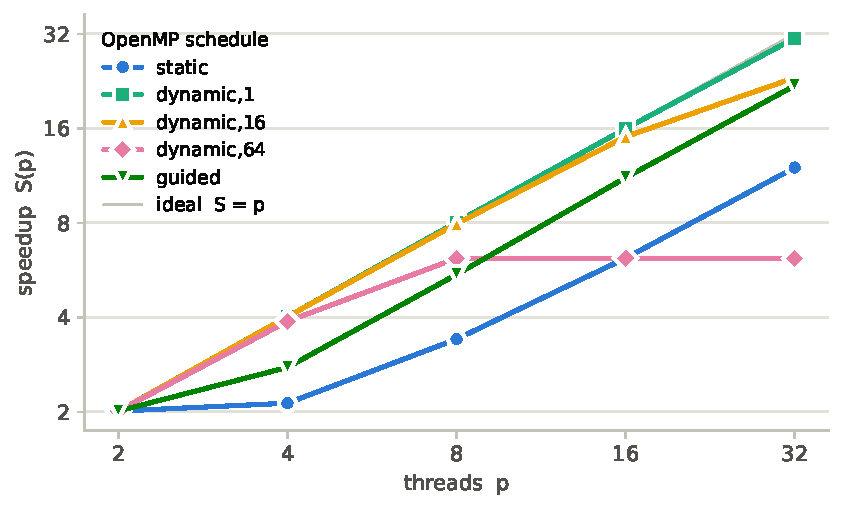
\includegraphics[width=0.85\textwidth]{Immagini/grafici/openmp_schedules}
    \caption{Speedup delle cinque politiche OpenMP in funzione del numero di
    thread, su assi logaritmici in base $2$, con la retta ideale $S = p$. I dati
    sono quelli della tabella~\ref{tab:openmp-schedule}.}
    \label{fig:openmp-schedules}
\end{figure}
\vspace{2,5mm}
Il dato d'insieme è la dispersione: a $32$ thread, sullo stesso hardware e sullo
stesso identico carico, la politica migliore è cinque volte più veloce della
peggiore. L'ordinamento a $p = 32$ è \texttt{dynamic,1} ($S = 30{,}99$),
\texttt{dynamic,16} ($23{,}21$), \texttt{guided} ($21{,}89$), \texttt{static}
($12{,}00$), \texttt{dynamic,64} ($6{,}17$). Poiché il lavoro da svolgere è
identico in tutti i casi --- stessa matrice, stesso checksum ---, il divario
dipende soltanto da come il lavoro è distribuito fra i thread: dall'inattività di
chi resta senza righe e, in misura minore, dal costo di coordinamento. A parità di
kernel, la scelta della politica vale dunque un fattore cinque.

\paragraph{La granularità può annullare il bilanciamento dinamico.}
Il caso più istruttivo della tabella è \texttt{dynamic,64}, che a $8$, $16$ e
$32$ thread restituisce lo stesso tempo a tre cifre significative
($0{,}11765$, $0{,}11746$, $0{,}11767$~s): raddoppiare e poi riquadruplicare i
thread non produce alcun guadagno. La spiegazione è quantitativa e si legge
nella tabella di previsione~\ref{tab:serial_pred_lambdaP}. Con chunk da $64$
righe su $1024$ esistono soltanto $16$ chunk, ciascuno dei quali è un blocco
contiguo; il makespan non può scendere sotto il chunk più pesante, e il peso del
più pesante fra $16$ blocchi contigui è precisamente ciò che misura $\lambda_p$
a $p=16$, da cui il tetto $6{,}169$. Il valore misurato è $6{,}167$. La soglia
cade dove la quota equa $\mathcal{W}/p$ scende sotto il chunk massimo, cioè
attorno a $p=7$: da lì in avanti aggiungere thread non cambia nulla, e a $32$
thread se ne stanno usando in pratica sei.

Se ne ricava una regola generale utile anche altrove: \emph{per uno scheduling
dinamico a chunk fissi di $c$ righe, il tetto allo speedup è quello della
decomposizione a blocchi con $H/c$ blocchi}, indipendentemente dal numero di
thread. Uno scheduling dinamico con grana troppo grossa degenera in uno
scheduling statico con pochi blocchi, e ne eredita per intero lo sbilanciamento
pagando in più il costo della coda.

\paragraph{Il chunk unitario e il costo del coordinamento.}
All'estremo opposto, \texttt{dynamic,1} raggiunge $30{,}99$ su $32$ thread, cioè
il $96{,}8\%$ dell'ideale, con $88{,}7$~GFLOP/s contro i $2{,}86$ del seriale.
Le $1024$ righe formano una coda abbastanza fine da assorbire completamente
l'irregolarità: la sua $e(p)$ resta sotto $0{,}0011$ ovunque, da uno a due
ordini di grandezza più piccola di quella dello statico. Il costo di coordinamento non è
però nullo, e diventa visibile proprio dove il bilanciamento è perfetto: fra
$p=16$ e $p=32$ l'efficienza scende da $0{,}999$ a $0{,}968$, ed è l'unico
punto della campagna in cui \texttt{dynamic,1} si scosta apprezzabilmente
dall'ideale. Con $1024$ prelievi da un contatore condiviso fra $32$ thread, la
contesa sulla coda comincia a farsi sentire. Il confronto con
\texttt{dynamic,16}, che a $32$ thread si ferma a $23{,}21$, mostra che il chunk
deve essere abbastanza piccolo da bilanciare: qui il guadagno di bilanciamento fra
$16$ righe e una riga supera il costo aggiuntivo della coda, perché il carico è
molto irregolare ($\mathrm{CoV} \approx 0{,}97$). Su un carico uniforme ci si
attenderebbe l'esito opposto, ed è questo il senso di $\mathrm{CoV}$ come
indicatore a priori.

\paragraph{\texttt{guided} perde per costruzione, non per overhead.}
La politica \texttt{guided} mostra un'efficienza notevolmente stabile
($0{,}693$, $0{,}685$, $0{,}697$, $0{,}684$ da $4$ a $32$ thread): perde circa
il $31\%$ e lo perde allo stesso modo a ogni grado di parallelismo. Un difetto
di overhead crescerebbe con $p$; una frazione seriale darebbe una $e(p)$
costante, mentre qui $e(p)$ decresce ($0{,}1475 \to 0{,}0149$). Il difetto è
strutturale: \texttt{guided} inizia assegnando chunk proporzionali
alle righe rimanenti, cioè blocchi contigui grandi, e i blocchi contigui in
questo problema ereditano la montagna centrale. I chunk fini, che sarebbero
quelli capaci di bilanciare, arrivano solo alla fine, quando non resta lavoro
con cui compensare. Il caso $p=4$ è il più netto: $2{,}773$ contro i $4{,}022$
di \texttt{dynamic,16}, un divario del $31\%$ fra due politiche entrambe
dinamiche. \texttt{guided} è progettata per ridurre l'overhead di coda su
carichi \emph{quasi} bilanciati; qui il carico è tutt'altro, e la sua euristica
lavora contro il problema.

\paragraph{Throughput assoluto.}
Le metriche viste finora sono tutte \emph{relative}: $S$, $E$ ed $e$ sono
rapporti a $T_1$, e per costruzione non dicono nulla su quanto valga $T_1$
stesso. Il throughput $\Pi(p)$ definito nella sezione~\ref{sec:lavoro}
è l'unica colonna assoluta della campagna, perché il numeratore
$F = \varphi\,\mathcal{W} = 2{,}077\cdot10^{9}$ FLOP è la medesima quantità
analitica per ogni variante --- discende dalla matrice degli escape time, non
dall'implementazione. A $32$ thread le cinque politiche danno

\begin{center}
\begin{tabular}{lrrrrr}
    \hline
    & \texttt{dynamic,1} & \texttt{dynamic,16} & \texttt{guided} & \texttt{static} & \texttt{dynamic,64} \\
    \hline
    $\Pi(32)$ [GFLOP/s] & $88{,}71$ & $66{,}45$ & $62{,}67$ & $34{,}35$ & $17{,}65$ \\
    \hline
\end{tabular}
\end{center}

\noindent contro i $2{,}86$~GFLOP/s del kernel seriale. Come metrica di scaling
$\Pi$ non aggiunge nulla --- il rapporto $\Pi(p)/\Pi(1)$ \emph{è} lo speedup,
per definizione --- ma rende visibile in valore assoluto ciò che la colonna $S$
esprime in rapporto, e soprattutto è la valuta comune con cui la
sezione~\ref{sec:cuda} confronterà CPU e GPU, dove il rapporto con il picco
teorico dell'hardware diventa la domanda centrale. Qui quel confronto non è
proponibile, perché il picco del nodo di calcolo non è stato caratterizzato, e
non lo si stima: $\Pi$ resta un termine di paragone \emph{fra le misure}, non
con il silicio.

Il caso che il throughput illustra meglio è \texttt{dynamic,64}, la cui curva
$\Pi$ si inchioda a $17{,}66$, $17{,}68$, $17{,}65$~GFLOP/s a $8$, $16$ e $32$
thread: il tetto di granularità discusso sopra, espresso in valore assoluto.

\paragraph{Lo statico satura il limite predetto.}
I dati di \texttt{static} si confrontano con il limite $p/\lambda_p$ calcolato
dal profilo seriale; la verifica quantitativa è riportata nella
sezione~\ref{sec:validazione-previsioni}, dove lo stesso confronto è esteso alle
decomposizioni MPI. Anticipando il risultato: l'accordo è entro lo $0{,}6\%$ su
tutti e cinque i punti, confermando che la perdita di efficienza è interamente
attribuibile allo sbilanciamento strutturale e non a overhead di OpenMP.

\paragraph{Lettura di Karp--Flatt.}
Delle tre firme classificate nella sezione~\ref{sec:metriche-comuni} le cinque
politiche ne esibiscono due soltanto, e l'assente è già un risultato: nessuna
mostra $e(p)$ \emph{costante}, cioè in nessun caso la perdita è imputabile a una
frazione seriale genuina --- coerentemente con un kernel che non ne contiene
alcuna. Tutto ciò che $e(p)$ registra qui è sbilanciamento oppure coordinamento,
e la direzione della metrica basta a separarli, purché la si legga insieme alla
forma del tetto e non da sola.
\vspace{2,5mm}
\begin{table}[htbp]
    \centering
    \begin{tabular}{llll}
        \hline
        Politica & $E(p)$, $p \ge 4$ & $e(p)$ & Meccanismo \\
        \hline
        \texttt{static}     & $0{,}533 \to 0{,}375$      & decresce, $0{,}2921 \to 0{,}0538$  & sbilanciamento strutturale \\
        \texttt{guided}     & $\approx 0{,}690$ costante & decresce, $0{,}1475 \to 0{,}0149$  & sbilanciamento strutturale \\
        \texttt{dynamic,1}  & $1{,}005 \to 0{,}968$      & cresce, $-0{,}0018 \to 0{,}0011$   & contesa sulla coda \\
        \texttt{dynamic,16} & $1{,}006 \to 0{,}725$      & cresce, $-0{,}0018 \to 0{,}0122$   & tetto di granularità \\
        \texttt{dynamic,64} & $0{,}971 \to 0{,}193$      & cresce, $0{,}0099 \to 0{,}1351$    & tetto di granularità \\
        \hline
    \end{tabular}
    \caption{OpenMP: classificazione delle cinque politiche secondo l'andamento
    di $e(p)$. L'efficienza è riportata sull'intervallo $p \ge 4$, che esclude
    il punto $p = 2$ affetto dallo scarto di $T_1$ discusso più avanti. Nessuna riga esibisce $e(p)$ costante: la frazione seriale
    nominale del kernel è nulla.}
    \label{tab:openmp-karp-flatt}
\end{table}

\medskip
\noindent\emph{Le politiche a $e(p)$ decrescente.}
\texttt{static} e \texttt{guided} condividono la stessa firma: un'efficienza che
si stabilizza su un valore $E_\infty < 1$ e una $e(p)$ che, sostituendo
$S = p\,E_\infty$ in~\eqref{eq:karp-flatt}, vale
\[
    e(p) = \frac{1/E_\infty - 1}{p - 1} \xrightarrow[p \to \infty]{} 0 .
\]
\texttt{guided} ne è l'esempio più puro, perché la sua efficienza è costante già
a $p = 4$ ($0{,}693$, $0{,}685$, $0{,}697$, $0{,}684$): con
$E_\infty = 0{,}690$ la formula predice $0{,}1500$, $0{,}0643$, $0{,}0300$,
$0{,}0145$ contro i misurati $0{,}1475$, $0{,}0658$, $0{,}0290$, $0{,}0149$. È
la conferma quantitativa di quanto osservato sopra: \texttt{guided} perde il
$31\%$ e lo perde allo stesso modo a ogni grado di parallelismo, il che è
incompatibile con un difetto di overhead.

Per \texttt{static} l'efficienza sta ancora scendendo verso il proprio asintoto
$1/\lambda = 0{,}362$, e conviene perciò usare la forma esatta. La politica
satura il proprio limite (sezione~\ref{sec:validazione-previsioni}), cioè
$S(p) = p/\lambda_p$, da cui
\[
    e(p) = \frac{\lambda_p - 1}{p - 1}
    \qquad
    (0{,}2933,\ 0{,}1927,\ 0{,}1062,\ 0{,}0536 \text{ per } p = 4, 8, 16, 32),
\]
che riproduce i valori misurati entro lo $0{,}5\%$. Poiché $\lambda_p$ è limitato
superiormente dal valore intrinseco $\lambda = 2{,}76$, anche qui la metrica
tende a \emph{zero}. Non c'è dunque alcun tetto fisso che lo statico stia
saturando: il valore $12{,}02$ è il limite \emph{alla singola taglia} $p = 32$,
non un asintoto, perché il tetto della decomposizione a blocchi vale
$p/\lambda_p$ e cresce con $p$, fino a $H/\lambda \approx 370$ nel caso limite
$p = H$. A distinguere i due casi è la \emph{direzione} della metrica, non il suo
valore: un tetto fisso $S_{\max}$ dà una $e(p)$ \emph{crescente}, che converge a
$1/S_{\max}$ dal basso --- è quanto si osserva più avanti per \texttt{dynamic,64}
--- mentre qui $e(p)$ decresce di un fattore cinque. Il confronto fra
$e(32) = 0{,}0538$ e $1/12{,}02 \approx 0{,}083$ non è di per sé dirimente,
perché anche un tetto fisso a $12{,}02$ lascerebbe $e(32)$ al di sotto di
$0{,}083$: è l'andamento, e solo l'andamento, a escludere il tetto.

\medskip
\noindent\emph{Le politiche a $e(p)$ crescente.}
Per \texttt{dynamic,1} la metrica parte da zero e cresce di pochissimo
($0{,}0011$ a $p = 32$): è il costo di coordinamento della coda condivisa, che
aumenta con il numero di thread che vi accedono. Non c'è qui alcun tetto ---
l'efficienza resta a $0{,}968$ --- e infatti i valori restano di due ordini di
grandezza sotto quelli delle politiche sbilanciate.

Le altre due politiche crescenti hanno invece un tetto, ed è lo stesso
meccanismo a due granularità diverse. La regola ricavata sopra --- chunk fissi
di $c$ righe ereditano il limite della decomposizione a blocchi con $H/c$
blocchi --- si applica anche a \texttt{dynamic,16}, che con $c = 16$ su $1024$
righe forma $64$ chunk. Interrogando a $P = 64$ lo stesso script di previsione
usato per la tabella~\ref{tab:serial_pred_lambdaP}
(\repofile{mandelbrot/analysis/block_imbalance.py}, opzione \texttt{-{}-p 64})
si ottiene $\lambda_{64} = 2{,}7076$, e quindi un tetto
$S_{\max} = 64/\lambda_{64} = 23{,}64$ contro i $23{,}21$ misurati a $32$
thread: uno scarto dell'$1{,}8\%$. Con quel tetto la forma chiusa dà
$e(32) = 0{,}0114$, contro lo $0{,}0122$ misurato. È la seconda verifica
indipendente della regola --- la prima essendo \texttt{dynamic,64} --- ed è
anche ciò che riclassifica la politica: il deficit di \texttt{dynamic,16} non è
contesa sulla coda, che con sedici volte più prelievi vale per
\texttt{dynamic,1} appena $0{,}0011$, ma granularità. Il tetto diventa vincolante
progressivamente, via via che la quota equa $\mathcal{W}/p$ scende sotto il peso
dei chunk più pesanti, ed è di fatto raggiunto a $p=32$: è per questo che
l'efficienza passa da $0{,}993$ a $8$ thread a $0{,}941$ a $16$ e a $0{,}725$ a
$32$.

\texttt{dynamic,64} è lo stesso meccanismo portato all'estremo, e vi si legge in
forma pura perché il tetto è già saturo dal primo punto misurato. I $16$ chunk
da $64$ righe non hanno un massimo ma \emph{due}, di peso identico ($2{,}59$
volte la media): il profilo di carico è simmetrico rispetto all'asse reale, e i
chunk delle righe $448$--$511$ e $512$--$575$ lo attraversano specularmente.
Ciascuno dei due pesa il $16{,}2\%$ di $\mathcal{W}$, e perché il makespan
scenda al tempo di uno di essi occorre che i restanti $p-2$ thread smaltiscano
gli altri quattordici chunk --- il $67{,}6\%$ del lavoro --- prima che quel
tempo sia trascorso, cioè $p \ge 6{,}17$: è la stessa soglia ricavata
sopra. Da lì in avanti lo speedup si inchioda
a $S_{\max} = 6{,}169$ e il makespan diventa praticamente indipendente da $p$
($p = 8$ è il primo punto misurato oltre la soglia, e vi si trova già a meno
dello $0{,}5\%$). Con $S$ costante in~\eqref{eq:karp-flatt} si ottiene
\[
    e(p) = \frac{1/S_{\max} - 1/p}{1 - 1/p}
    \qquad
    (0{,}0424,\ 0{,}1062,\ 0{,}1351 \text{ per } p = 8, 16, 32),
\]
che converge al reciproco $1/S_{\max} \approx 0{,}162$ \emph{dal basso}.

È la classificazione della sezione~\ref{sec:metriche-comuni} osservata sui dati:
le due politiche peggiori dello sweep, \texttt{static} e \texttt{dynamic,64},
stanno agli estremi opposti pur fallendo entrambe, ed è l'andamento di $e(p)$ a
distinguerne la causa.

\paragraph{Due avvertenze sulla lettura dei dati.}
A $p=2$ tutte e cinque le politiche danno $S \approx 2{,}011$, cioè leggermente
\emph{superlineare}, con $E > 1$ e $e(p)$ negativa. Lo scarto è di $4$~ms su
$726$ ed è identico su tutte le politiche, quindi non è un effetto di
scheduling: la causa è la variabilità di $T_1$ stesso fra job distinti. Lo
stesso binario seriale, sulla stessa configurazione e sullo stesso nodo, misura
$0{,}72563$~s nel job OpenMP e $0{,}72233$~s nel job della baseline
(tabella~\ref{tab:serial_var_Nmax}): $3{,}3$~ms di differenza, cioè da sola
quasi tutta l'eccedenza. Adottando la seconda misura lo speedup a $p = 2$ scende
a $2{,}002$ e la superlinearità sparisce. Il valore non va dunque interpretato
come un guadagno superlineare genuino, ma come il rumore residuo fra job
distinti su un nodo condiviso.

La tabella conserva comunque il $T_1$ misurato nello stesso job dei
$T_\parallel(p)$: stesso job significa stesso nodo nello stesso stato, mentre
adottare la misura più veloce fra job diversi nasconderebbe l'anomalia
scegliendo il denominatore più comodo. Per la stessa ragione lo script di merge
abbina ogni misura alla baseline del proprio job: con il minimo globale, l'arrivo
dello sweep MPI ($T_1 = 0{,}72021$~s) avrebbe spostato dello $0{,}75\%$ tutti gli
speedup di questa tabella senza che alcuna misura OpenMP fosse ripetuta.

La seconda avvertenza riguarda il rumore di sistema e giustifica a posteriori la
scelta del minimo su ripetizioni. Per \texttt{guided} a $32$ thread il tempo
medio sulle cinque ripetizioni è $0{,}0496$~s contro un minimo di $0{,}0331$~s e
una mediana di $0{,}0339$~s: la media supera il minimo del $50\%$, ma è la
mediana a rivelare la struttura del disturbo. Quattro ripetizioni su cinque
stanno attorno al minimo, e perché la media salga a $0{,}0496$~s la quinta deve
essere durata circa $0{,}11$~s, cioè \emph{tre volte e mezzo} il minimo: un
singolo episodio isolato e non un rallentamento diffuso, presumibilmente per
contesa su banda di memoria o cache di ultimo livello con un altro job presente
sul nodo. La media avrebbe attribuito a \texttt{guided} un difetto che non ha;
il minimo, essendo il rumore additivo, ha isolato il tempo di calcolo genuino.

\paragraph{Sintesi.}
Il filo \emph{predetto contro misurato} si chiude su tre livelli. La correttezza
è verificata dal checksum, identico su tutte e $26$ le righe e coincidente con
quello della baseline seriale: nessuna politica ha alterato il risultato, il che
conferma sperimentalmente l'assenza di corse in scrittura. Lo sbilanciamento
predetto in sede seriale è verificato dalla saturazione dello statico sul
proprio limite entro lo $0{,}6\%$, come dettagliato nella
sezione~\ref{sec:validazione-previsioni}. E il valore diagnostico del
$\mathrm{CoV} \approx 0{,}97$ è confermato dal fatto che lo scheduling dinamico
a grana fine, che su un carico uniforme sarebbe stato uno spreco, recupera qui
quasi per intero il $62\%$ di efficienza che la decomposizione statica perde.

Resta aperta una domanda che questa sottosezione non può chiudere da sola:
quanto di ciò che si è visto dipenda dalla \emph{politica} e quanto dal
\emph{modello di memoria}. La risposta richiede di eseguire la stessa identica
politica sotto un paradigma diverso, ed è il confronto che la
sezione~\ref{sec:mpi-risultati} conduce mettendo \texttt{dynamic,1} a fronte del
master--worker MPI a concessione unitaria, sullo stesso nodo
(tabella~\ref{tab:dynamic-confronto}). Anticipandone l'esito: i due meccanismi si
equivalgono entro circa l'$1\%$ a $32$ unità, e il divario che
resta non è di prestazioni ma di complessità implementativa.
%--------------------- MPI -------------------
% Sezione completa: sweep eseguito (job 34137, gnode01, 2026-09-09), dati in
% mandelbrot/data/run_34137.csv e mandelbrot/data/merged.csv.
% I limiti p/lambda_p provengono da mandelbrot/data/block_imbalance.csv.
\subsection{MPI: memoria distribuita}
\label{sec:mpi}

Il passaggio a MPI cambia il vincolo fondamentale, non la decomposizione. La
grana resta la riga, per le stesse ragioni della sezione~\ref{sec:openmp}, ma i
processi non condividono più uno spazio di indirizzamento: ciascun rank possiede
una propria copia parziale della matrice degli escape time, e il risultato
completo esiste solo dopo un atto esplicito di comunicazione. Ne discendono le
due differenze che governano l'intera sottosezione. Primo, la matrice va
\emph{assemblata}: nei due schemi statici con una \texttt{MPI\_Gatherv} finale
su rank $0$, nello schema dinamico incrementalmente, riga per riga, man mano che
i risultati arrivano. Secondo, e più importante, il ribilanciamento del carico
non è più gratuito: sotto OpenMP un thread inattivo prelevava lavoro da una coda
in memoria condivisa a costo trascurabile, mentre qui ogni atto di
ridistribuzione è un messaggio, potenzialmente attraverso la rete. È questo
prezzo a rendere il confronto fra schemi la vera domanda del paradigma.

Il parallelismo resta quello per righe, ma l'unità è ora il processo e non il
thread; il numero di unità di calcolo è spazzato sugli stessi valori
($2, 4, 8, 16, 32$) usati per OpenMP, e griglia e $N_{\max}$ restano fissi
($1024^2$, $1000$), così che il confronto fra paradigmi avvenga sullo stesso
carico di lavoro. Non si sfrutta la simmetria, coerentemente con tutti gli altri
benchmark di scaling: dimezzerebbe il lavoro senza cambiare la matrice
risultante, ma renderebbe metà delle righe una copia anziché un calcolo,
falsando il profilo $\{w_r\}$ su cui poggia l'intera analisi di sbilanciamento.

% ============================================================
\subsubsection{Design dello sweep}
\label{sec:mpi-sweep}
% ============================================================

La domanda progettuale non è quanto parallelizzare, ma \emph{con quale regola
assegnare le righe ai rank}. A differenza di OpenMP, dove la scelta era fra
politiche di scheduling dello stesso pool di thread, qui le regole differiscono
anche nel volume di comunicazione che generano: è possibile bilanciare meglio
pagando più messaggi, oppure bilanciare altrettanto bene senza aggiungerne.
Questo asse è ciò che i tre schemi esplorano.

\paragraph{\texttt{block}.}
Il rank $r$ possiede un intervallo contiguo di $H/p$ righe. La
distribuzione è nota a tutti prima di iniziare: non esiste dialogo, e la
comunicazione si riduce a un'unica \texttt{MPI\_Gatherv} finale. Poiché, per la
viewport scelta, il corpo del frattale occupa le righe centrali della griglia e
le righe di bordo contengono solo punti esterni che sfuggono in poche
iterazioni, i rank centrali concentrano quasi tutto il lavoro. La riga più
leggera è la riga $0$ ($2\,281$ iterazioni totali, circa $2$ per pixel) e la
più pesante la riga $511$, al centro ($700\,806$, circa $684$ per pixel): un
rapporto di $307\times$. I rank che ricevono il primo e l'ultimo blocco sono
necessariamente veloci per costruzione; i rank centrali portano da soli la
maggior parte del lavoro. È il caso di massimo sbilanciamento con comunicazione
minima, e il suo limite $S \le p/\lambda_p$ è calcolabile dal solo profilo
seriale prima ancora che il codice MPI esista.

\paragraph{\texttt{cyclic}.}
La riga $r$ va al rank $r \bmod p$. Ogni rank riceve righe sparse su tutta
l'immagine --- un po' di bordo, un po' di centro --- e il carico si media da sé,
perché il pattern di fuga varia su una scala spaziale molto più grande della
singola riga. L'assegnazione resta \emph{statica}: ogni rank sa già quali righe
possiede, non esiste coda residua, e la comunicazione è la stessa unica gather
del block --- a meno di un riordino locale su rank $0$ per de-interlacciare il
buffer, che non è un messaggio ma non è nemmeno gratuito, come mostreranno i
risultati.

Ciò che rende il cyclic interessante non è soltanto che batta il block: è che
\emph{esce dall'asse} bilanciamento--comunicazione su cui si trova il dinamico.
Lungo quell'asse, ridurre il chunk avvicina al bilanciamento ma moltiplica i
messaggi; il cyclic ottiene un bilanciamento quasi equivalente al dinamico con
zero messaggi aggiuntivi, perché è l'interlacciamento statico a mediare il
carico, non la coordinazione a runtime. La domanda aperta che l'esperimento deve
rispondere è se questo vantaggio sia sufficiente a battere o pareggiare il
master--worker nonostante il riordino.

\paragraph{\texttt{dynamic} (master--worker).}
Il rank $0$ non calcola nulla: tiene le righe non distribuite come coda di
lavoro, innesca ciascun worker con una riga e poi alimenta con la successiva il
primo worker che riporta un risultato. L'assegnazione si adatta al costo reale
di ogni riga --- chi è bloccato su una riga pesante semplicemente non viene
rifornito --- e il bilanciamento è perfetto per costruzione. Il prezzo è una
coppia di messaggi richiesta/risposta per ogni riga. Questo schema è il limite
opposto al block: bilanciamento massimo, overhead di comunicazione massimo.

È importante notare che, al crescere del chunk, il master--worker non degenera
nel cyclic ma nel block: con chunk pari a $H/p$ righe, dove $p$ è il numero di
worker, ogni worker riceve un unico
blocco contiguo, che è esattamente la decomposizione a blocchi contigui. Il
cyclic non è un punto sull'asse chunk--overhead: è un meccanismo ortogonale che
non occupa alcuna posizione su quell'asse.

\paragraph{Grana della concessione e conteggio delle unità.}
La concessione è fissata a una riga, senza sweep sul chunk, per tre ragioni.
Un chunk intermedio si colloca fra estremi già misurati: comunica più del
cyclic, che non aggiunge messaggi, e bilancia meno del chunk unitario. In secondo luogo l'estremo è il
punto più informativo: accoppia il miglior bilanciamento possibile con il massimo
costo di coordinamento, ed è precisamente il confronto che lo schema esiste per
esporre. Infine l'asse del chunk è già spazzato dove costa poco, nei run OpenMP
\texttt{dynamic,\{1,16,64\}}; tenendo il chunk unitario da entrambi i lati, i
due scheduler dinamici diventano la stessa politica su due modelli di memoria
diversi, e il loro divario isola il costo del passaggio di messaggi rispetto
all'incremento di un contatore condiviso.

Poiché il master non calcola, per lo schema dinamico $p$ indica il numero di
\emph{worker} e non di processi: gli sweep girano su $np \in \{3, 5, 9, 17,
33\}$ per mantenere le unità di calcolo a $\{2, 4, 8, 16, 32\}$, allineate agli
altri schemi e ai thread OpenMP. Va dichiarato che la contabilità è leggermente
generosa verso il master--worker: il cluster alloca $p+1$ core, uno dei quali
non calcola; speedup ed efficienza sono per unità di calcolo, e il costo reale
in risorse è $p+1$ processi.

% ============================================================
\subsubsection{Metriche specifiche}
\label{sec:mpi-metriche}
% ============================================================

Alle metriche comuni della sezione~\ref{sec:metriche-comuni} MPI aggiunge una
grandezza propria: la \emph{frazione di comunicazione}, cioè la quota di $T_\parallel(p)$
spesa a muovere dati anziché a calcolare. È la metrica che dà corpo al costo
introdotto dalla memoria distribuita, e la sua definizione operativa differisce
fra schemi statici e dinamico.

Negli schemi statici la comunicazione è un unico \texttt{MPI\_Gatherv} finale, e
il suo tempo è misurato \emph{dopo} una barriera. La scelta è deliberata: senza
barriera il rank in ritardo farebbe apparire dentro la gather l'attesa dovuta
allo sbilanciamento, gonfiando \texttt{comm\_fraction} con un tempo che non è
trasferimento di dati. Con la barriera l'inattività resta parcheggiata prima
dell'operazione --- e comunque dentro la regione cronometrata, quindi $T_\parallel(p)$
resta onesto --- mentre \texttt{comm\_fraction} misura solo movimento genuino di
dati. Lo sbilanciamento è riportato altrove, da $\lambda_p$ e dallo speedup; e
tenere le due cose separate è ciò che rende leggibile il confronto.

Nello schema dinamico la definizione è necessariamente diversa. Il master
comunica il $100\%$ del tempo per costruzione --- è la sua sola funzione ---
quindi il suo tempo non direbbe nulla sulla frazione di coordinamento pagata
\emph{dal calcolo}. Si misura invece, per ciascun worker, la frazione del proprio
tempo trascorsa dentro le chiamate MPI: l'invio del risultato di una riga e
l'attesa bloccante del comando successivo. Questa attesa è inclusa
deliberatamente, perché contiene sia la latenza del messaggio sia la contesa
quando più worker riportano insieme --- che è precisamente il prezzo della
coordinazione dinamica. Il valore medio dei worker è raccolto con una
\texttt{MPI\_Reduce} su rank $0$ e riportato come \texttt{comm\_fraction}. È
l'unico degli schemi per cui questa colonna diventa una metrica significativa:
negli statici la frazione è attesa prossima a zero e serve come controllo, nel
dinamico è il numero che quantifica il costo del self-scheduling.

% ============================================================
\subsubsection{Frammenti di codice rilevanti}
\label{sec:mpi-codice}
% ============================================================

Come per OpenMP, un solo binario copre tutti gli schemi: la variabile d'ambiente
\texttt{MPI\_DECOMP} seleziona a esecuzione fra \texttt{block}, \texttt{cyclic}
e \texttt{dynamic} (default \texttt{block}), e il job passa l'etichetta
corrispondente a \texttt{-{}-schedule} per il CSV. Il codice completo del kernel
si trova nel file \repofile{mandelbrot/src/mandelbrot_mpi.cpp}, mentre lo strato
driver descritto più avanti si trova nel file \repofile{mandelbrot/src/main.cpp}.

La differenza fra i due schemi statici è una sola espressione --- quale riga
globale corrisponda all'$i$-esima riga locale:

\begin{verbatim}
// block:  global row = row_displs[rank] + i   (contiguous range)
// cyclic: global row = rank + i*size          (strided)
const int row = (decomp == Decomp::Block) ? (row_displs[rank] + i)
                                          : (rank + i * size);
\end{verbatim}

È il frammento più significativo della sottosezione: il cyclic ottiene gran
parte del bilanciamento del master--worker cambiando un indice. I conteggi di
righe per rank sono identici nei due casi (\texttt{base} righe ciascuno, le
prime \texttt{rem} ne prendono una in più); cambia solo \emph{quali} righe un
rank possiede. Il block raccoglie direttamente nella matrice finale, essendo i
suoi dati già contigui; il cyclic raccoglie in un buffer compattato che il rank
$0$ poi de-interlaccia, un riordino locale in memoria che non aggiunge alcun
messaggio. La simmetria fra i due schemi è però meno perfetta di quanto la
singola espressione suggerisca: quel riordino è una copia seriale dell'intera
matrice, eseguita da un solo rank e di costo indipendente da $p$. Non entra in
\texttt{comm\_fraction} --- non è comunicazione --- ma entra in $T_\parallel(p)$,
ed è l'unico costo del cyclic assente negli altri due schemi; se ne discute
il peso nell'analisi dei risultati. Sarebbe eliminabile ricevendo direttamente
in posizione con un tipo derivato \texttt{MPI\_Type\_vector} di passo
\texttt{size}, al prezzo di una gather su tipo non contiguo.

La gather è cronometrata dopo una barriera, per la ragione discussa sopra:

\begin{verbatim}
MPI_Barrier(MPI_COMM_WORLD);      // park the straggler wait outside the timing
const double t0 = MPI_Wtime();    // of the gather (but inside T(p))
MPI_Gatherv(local.data(), my_rows * width, MPI_INT, recvbuf,
            px_counts.data(), px_displs.data(), MPI_INT, 0, MPI_COMM_WORLD);
g_last_comm_seconds = MPI_Wtime() - t0;
\end{verbatim}

Lo schema dinamico è invece l'unico che richiede un'architettura dedicata. Il
protocollo è minimale: il comando è un intero (l'indice di riga), il risultato è
\texttt{width+1} interi --- l'indice di riga seguito dagli escape time di quella
riga --- cosicché il master archivi il risultato all'arrivo senza tenere traccia
di chi detenga cosa. Il cuore è il ciclo di eventi del master:

\begin{verbatim}
while (active > 0) {
    MPI_Recv(result.data(), width + 1, MPI_INT, MPI_ANY_SOURCE, TAG_RESULT,
             MPI_COMM_WORLD, &status);        // whoever finishes first
    // file the row into the matrix, then feed that same worker
    if (next_row < height) {
        MPI_Send(&next_row, 1, MPI_INT, status.MPI_SOURCE, TAG_WORK, ...);
        ++next_row;
    } else {
        MPI_Send(&none, 1, MPI_INT, status.MPI_SOURCE, TAG_STOP, ...);
        --active;
    }
}
\end{verbatim}

\texttt{MPI\_ANY\_SOURCE} è ciò che realizza il self-scheduling: non è il master
a decidere chi lavora, ma il primo worker che si libera a farsi avanti. La
terminazione è implicita: ogni worker attivo detiene esattamente una riga in
sospeso, quindi \texttt{active} si annulla quando tutte le righe
sono state ricevute. Non serve alcuna gather finale, perché la matrice si compone
incrementalmente sul master. Vale la pena notare il contrasto con OpenMP: lì la
coda era un dettaglio interno al runtime, invisibile nel codice utente; qui la
stessa politica richiede un protocollo di messaggi esplicito, un master dedicato
e una condizione di terminazione da dimostrare. È il costo di complessità, prima
ancora che di tempo.

\paragraph{Strato driver.}
MPI richiede un sottile adattamento del driver condiviso, isolato dietro
\texttt{\#ifdef USE\_MPI} così da lasciare invariate le build seriale e OpenMP:
inizializzazione e chiusura di MPI, una barriera che allinea l'inizio della
regione cronometrata su tutti i rank, e l'I/O confinato al rank $0$, l'unico a
detenere la matrice assemblata. Il tempo di comunicazione raggiunge il CSV
attraverso l'accessore \texttt{kernel\_comm\_seconds()}, nullo per seriale e
OpenMP, senza che il kernel calcoli metriche.

\paragraph{Configurazione della misura: un solo nodo, per vincolo.}
Il job gira su un \textbf{unico nodo}, per un vincolo dell'ambiente e non per
scelta metodologica (sezione~\ref{sec:ambiente}): una richiesta con
\texttt{-{}-nodes=2} viene rifiutata da SLURM al momento della sottomissione. Il
paradigma nato per la memoria distribuita viene
dunque misurato, per forza di cose, su memoria condivisa.

L'allocazione è di $33$ task su un nodo, con i rank ancorati ai core e assegnati
in ordine, riempiendo un socket prima di passare all'altro
(\texttt{-{}-map-by core -{}-bind-to core}). È l'analogo MPI del
\texttt{OMP\_PROC\_BIND=close} usato per OpenMP: senza, il runtime potrebbe
distribuire i due soli rank di $p=2$ su socket diversi, caricando i punti a
basso $p$ di una penalità inter-socket estranea alla decomposizione. Soltanto a
$np=33$ un rank risiede necessariamente sul secondo socket. Si noti che questo posizionamento \emph{rank\,$\to$\,core}
è cosa distinta dalla decomposizione \emph{riga\,$\to$\,rank} che porta lo stesso
nome ``a blocchi''.

La conseguenza va dichiarata apertamente. Tutti i messaggi transitano per la
memoria condivisa del nodo e non per la rete, dunque la
\texttt{comm\_fraction} misurata è un \emph{limite inferiore ottimistico}
rispetto a quanto pagherebbe un'esecuzione realmente distribuita: quantifica
correttamente \emph{quanta} comunicazione ciascuno schema richiede, ma ne
sottostima il prezzo unitario. Il divario fra master--worker e schemi statici va
perciò letto come ottimistico verso il primo. In cambio si ottiene che $T_1$ e
$T_\parallel(p)$ sono garantiti sullo stesso hardware per costruzione, e che le
curve MPI e OpenMP diventano direttamente confrontabili nei valori assoluti, non
solo nelle tendenze: la loro differenza riflette in larga misura il solo
modello di programmazione.

\paragraph{Il lanciatore: \texttt{mpirun} e non \texttt{srun}.}
La versione di OpenMPI disponibile sul cluster non può essere lanciata
direttamente da \texttt{srun}: con il modulo \texttt{amd/gcc-8.5.0/openmpi-4.1.6}
ogni rank termina dentro \texttt{MPI\_Init} con l'errore
\begin{verbatim}
OPAL ERROR: Unreachable in file ext3x_client.c at line 111
\end{verbatim}
La causa è un disallineamento di versione nello strato di avvio: il client PMIx
di OpenMPI~$4.1.6$ è costruito per PMIx~$3.x$ e non dialoga con il server PMIx
v5 esposto da SLURM. I rank sono quindi lanciati con \texttt{mpirun}, che legge
l'allocazione dalle variabili d'ambiente di SLURM e avvia i processi con il PMIx
interno a OpenMPI. Il posizionamento dei rank resta invariato
(\texttt{-{}-map-by core -{}-bind-to core}), mentre la variabile
\texttt{MPI\_DECOMP} va inoltrata esplicitamente con \texttt{-x}, perché
\texttt{mpirun} propaga di default le sole variabili \texttt{OMPI\_*}. La
baseline seriale, che non usa MPI, continua a essere lanciata con \texttt{srun}.

Restano valide le scelte già motivate per OpenMP e per l'ambiente di misura
(sezione~\ref{sec:ambiente}): $T_1$ misurato con il binario seriale vero sullo
stesso nodo, compilazione dentro il job, kernel \emph{bare} come riferimento di
scaling.

% ============================================================
\subsubsection{Analisi dei risultati}
\label{sec:mpi-risultati}
% ============================================================

% Dati: job 34137 su gnode01, partizione ulow, 53 s di elapsed, COMPLETED 0:0.
% run_34137.csv (15 punti MPI + la propria baseline seriale) e merged.csv.
% T(1) = 0,720205 s, misurato nello stesso job.

Il confronto mette a sistema i tre schemi sullo stesso intervallo di unità di
calcolo, a griglia e $N_{\max}$ fissati. La tabella~\ref{tab:mpi-schemi}
raccoglie i $15$ punti misurati.\footnote{Job $34137$ su \texttt{gnode01},
    partizione \texttt{ulow}. Gli speedup sono riferiti alla baseline seriale
    misurata \emph{dentro lo stesso job}, $T_1 = 0{,}72021$~s; lo sweep OpenMP usa
    analogamente la propria, $0{,}72563$~s. Le due differiscono dello $0{,}75\%$, che
    è il fondo di risoluzione di qualunque confronto \emph{fra} paradigmi condotto
    sugli speedup: per questo il raffronto diretto con OpenMP, più avanti, è fatto
    sui tempi.}
\vspace{2,5mm}
\begin{table}[htbp]
    \centering
    \begin{tabular}{llrrrrrr}
        \hline
        Schema & $p$ & $S \le p/\lambda_p$ & $T_\parallel(p)$ [s] & $S(p)$ & $E(p)$ & $e(p)$ & comm.\ [\%] \\
        \hline
        seriale  & 1  & ---     & $0{,}72021$ & --- & --- & --- & --- \\
        \hline
        block    & 2  & $2{,}00$  & $0{,}36113$ & $1{,}994$  & $0{,}997$ & $0{,}0029$ & $0{,}13$ \\
        block    & 4  & $2{,}13$  & $0{,}33965$ & $2{,}120$  & $0{,}530$ & $0{,}2955$ & $0{,}08$ \\
        block    & 8  & $3{,}41$  & $0{,}21255$ & $3{,}388$  & $0{,}424$ & $0{,}1944$ & $0{,}14$ \\
        block    & 16 & $6{,}17$  & $0{,}11759$ & $6{,}125$  & $0{,}383$ & $0{,}1075$ & $0{,}31$ \\
        block    & 32 & $12{,}02$ & $0{,}06157$ & $11{,}697$ & $0{,}366$ & $0{,}0560$ & $1{,}20$ \\
        \hline
        cyclic   & 2  & $2{,}00$  & $0{,}36252$ & $1{,}987$  & $0{,}993$ & $0{,}0067$ & $0{,}18$ \\
        cyclic   & 4  & $4{,}00$  & $0{,}18126$ & $3{,}973$  & $0{,}993$ & $0{,}0022$ & $0{,}25$ \\
        cyclic   & 8  & $7{,}99$  & $0{,}09096$ & $7{,}918$  & $0{,}990$ & $0{,}0015$ & $0{,}24$ \\
        cyclic   & 16 & $15{,}97$ & $0{,}04930$ & $14{,}608$ & $0{,}913$ & $0{,}0064$ & $3{,}37$ \\
        cyclic   & 32 & $31{,}70$ & $0{,}02411$ & $29{,}871$ & $0{,}933$ & $0{,}0023$ & $3{,}02$ \\
        \hline
        dynamic  & 2  & $2{,}00$  & $0{,}36199$ & $1{,}990$  & $0{,}995$ & $0{,}0053$ & $0{,}43$ \\
        dynamic  & 4  & $4{,}00$  & $0{,}18154$ & $3{,}967$  & $0{,}992$ & $0{,}0028$ & $0{,}68$ \\
        dynamic  & 8  & $8{,}00$  & $0{,}09092$ & $7{,}921$  & $0{,}990$ & $0{,}0014$ & $0{,}86$ \\
        dynamic  & 16 & $16{,}00$ & $0{,}04622$ & $15{,}583$ & $0{,}974$ & $0{,}0018$ & $2{,}21$ \\
        dynamic  & 32 & $32{,}00$ & $0{,}02316$ & $\mathbf{31{,}102}$ & $0{,}972$ & $0{,}0009$ & $2{,}54$ \\
        \hline
    \end{tabular}
    \caption{MPI: metriche per schema di decomposizione e numero di unità di
    calcolo. Griglia $1024^2$, $N_{\max}=1000$, $33$ rank su un unico nodo. Per lo
    schema dinamico $p$ indica i worker; i processi allocati sono $p+1$. La colonna
        $S \le p/\lambda_p$ riporta il limite predetto a priori dal profilo di carico
        seriale (tabella~\ref{tab:serial_pred_lambdaP}) e non è una misura: è il termine
        di confronto contro cui va letto lo speedup osservato.}
    \label{tab:mpi-schemi}
\end{table}
\vspace{2,5mm}
\begin{table}[htbp]
    \centering
    \begin{tabular}{lrrrr}
        \hline
        $p$ & $T$ OpenMP \texttt{dynamic,1} [s] & $T$ MPI \texttt{dynamic} [s] &
        divario & comm.\ MPI [\%] \\
        \hline
        2  & $0{,}36079$ & $0{,}36199$ & $+0{,}33\%$ & $0{,}43$ \\
        4  & $0{,}18043$ & $0{,}18154$ & $+0{,}62\%$ & $0{,}68$ \\
        8  & $0{,}09028$ & $0{,}09092$ & $+0{,}71\%$ & $0{,}86$ \\
        16 & $0{,}04542$ & $0{,}04622$ & $+1{,}76\%$ & $2{,}21$ \\
        32 & $0{,}02342$ & $0{,}02316$ & $-1{,}11\%$ & $2{,}54$ \\
        \hline
    \end{tabular}
    \caption{Confronto dei due scheduler dinamici a parità di politica (concessione
    di una riga): stessa strategia su modelli di memoria diversi. Il confronto è sui
    \emph{tempi} e non sugli speedup, così da essere indipendente dalla baseline
    seriale usata dai due sweep. Divario positivo significa MPI più lento. Si ricordi
    che a $p$ unità di calcolo MPI occupa $p+1$ core, OpenMP $p$.}
    \label{tab:dynamic-confronto}
\end{table}

\paragraph{Il quadro d'insieme.}
A $32$ unità di calcolo, sullo stesso hardware e sullo stesso carico, lo speedup
va da $11{,}70$ (block) a $31{,}10$ (master--worker): un fattore $2{,}66$ fra la
regola peggiore e la migliore, che coincide entro lo $0{,}1\%$ con lo
sbilanciamento $\lambda_{32}$ previsto per i blocchi dal solo profilo seriale.
Il rapporto fra speedup misurato e limite previsto è compreso fra $0{,}972$ e
$0{,}997$ in tredici punti su quindici; le due eccezioni sono il cyclic a $p=16$
e $p=32$ ($0{,}915$ e $0{,}942$), discusse più avanti. Il confronto punto per
punto, esteso a OpenMP, è nella sezione~\ref{sec:validazione-previsioni}.

\paragraph{Il block è limitato dal proprio $\lambda_p$.}
Il dato più vistoso della tabella è il passaggio da $p=2$ a $p=4$: raddoppiando
i processi il tempo scende da $0{,}36113$~s a $0{,}33965$~s, cioè del $6\%$.
Non è un'anomalia di misura: è $\lambda_p$ che passa da $1{,}0000$ a $1{,}8798$
e si mangia per intero il raddoppio. Il punto $p=2$ merita una nota, perché è
ingannevole: la sua efficienza quasi perfetta ($0{,}997$) non dice che il block
scali bene a $p$ piccolo, ma che la viewport è simmetrica rispetto all'asse
reale, sicché le due metà dell'immagine contengono esattamente lo stesso numero
di iterazioni ($129\,827\,745$ ciascuna) e $\lambda_2 = 1$ per una proprietà
geometrica dell'insieme, non della decomposizione.

Al crescere di $p$ il $\lambda_p$ dei blocchi continua a crescere, fino al valore
intrinseco $\lambda = 2{,}76$ del caso limite $p = H$. L'efficienza tende perciò
a stabilizzarsi attorno a $1/\lambda_p$, pari a $0{,}376$ a $p=32$ contro lo
$0{,}366$ misurato, mentre lo speedup continua a crescere: già a $p=32$, però,
circa il $63\%$ del tempo di calcolo aggregato va perso in attesa.

\paragraph{Lettura di Karp--Flatt.}
Il block è il caso di scuola in cui la metrica segnala correttamente un problema
attribuendolo però alla causa sbagliata. Se il deficit fosse una frazione
seriale alla Amdahl, $e(p)$ sarebbe costante; qui invece decresce di un fattore
cinque, da $0{,}2955$ a $0{,}0560$, e segue la forma
$e(p) \approx (\lambda_p - 1)/(p - 1)$ già ricavata per lo \texttt{static} di
OpenMP (sezione~\ref{sec:openmp-risultati}), che realizza la stessa regola: i
valori predetti, $0{,}2933$, $0{,}1927$, $0{,}1062$ e $0{,}0536$ per
$p = 4, 8, 16, 32$, riproducono i misurati entro l'$1\%$ fino a $p=16$; a
$p=32$ lo scarto sale al $4{,}5\%$, nello stesso punto in cui lo speedup si
allontana dal limite. La ``frazione seriale
sperimentale'' non misura codice seriale, ma sbilanciamento.

\paragraph{Block e cyclic: bilanciamento a costo zero.}
Il primo confronto isola il puro effetto del bilanciamento: la comunicazione è
la stessa unica gather, dunque ogni differenza di tempo è attribuibile alla sola
distribuzione delle righe. Fino a $p=8$ il cyclic è indistinguibile dall'ideale
--- $E = 0{,}993$, $0{,}993$, $0{,}990$ a $2$, $4$ e $8$ processi --- mentre il
block, sulla stessa gather e sullo stesso carico, si ferma a $0{,}997$, $0{,}530$
e $0{,}424$. A $p=8$ il rapporto fra i due tempi è $2{,}34$, contro il $2{,}35$
predetto dal rapporto dei rispettivi $\lambda_p$: l'intero divario è
distribuzione delle righe. La \texttt{comm\_fraction} chiude l'argomento: $0{,}18\%$,
$0{,}25\%$, $0{,}24\%$ per il cyclic contro $0{,}13\%$, $0{,}08\%$, $0{,}14\%$
per il block, cioè fra $0{,}2$ e $0{,}7$~ms in entrambi i casi --- la stessa cosa
entro il rumore di misura. Non c'è stato alcun dialogo aggiuntivo: solo la
medesima gather finale. L'equivalenza vale però soltanto su questo intervallo di
$p$, e si rompe a $p=16$: se ne discute subito sotto.

\paragraph{Il master--worker e il costo del coordinamento.}
Il master--worker firma il miglior punto assoluto dell'intera campagna CPU:
$S = 31{,}10$ su $32$ unità di calcolo, $E = 0{,}972$, $89{,}7$~GFLOP/s contro i
$2{,}88$ della baseline seriale. Il residuo del $2{,}8\%$ è comunicazione, e la
colonna che lo misura è già in tabella. Confrontando riga per riga il deficit
dal limite $p/\lambda_p$ con la \texttt{comm\_fraction} si ottiene $0{,}5\%$
contro $0{,}43\%$ a $p=2$, poi $0{,}8$ contro $0{,}68$, $1{,}0$ contro $0{,}86$,
$2{,}6$ contro $2{,}21$ e $2{,}8\%$ contro $2{,}54\%$ a $p=32$: i due andamenti
coincidono entro pochi decimi di punto su tutti e cinque i punti. Lo stesso
numero si ricava per via indipendente dal protocollo: a $p=32$ un worker spende
circa $18~\mu$s di round-trip per riga contro $0{,}70$~ms di calcolo medio, cioè
il $2{,}6\%$ del proprio tempo. La coincidenza non è casuale ma strutturale:
poiché il bilanciamento è perfetto ($\lambda_p = 1$) e il tempo di un worker è
calcolo più attesa, il deficit dal limite \emph{è} la frazione di comunicazione,
e non resta un residuo da attribuire ad altro.

Vale la pena escludere esplicitamente la spiegazione alternativa, perché è quella
che il modello del makespan suggerirebbe. Il lavoro non è frazionabile a piacere:
l'unità indivisibile è la riga, e l'ultima riga consegnata a un worker potrebbe
in linea di principio essere la più pesante, lasciando gli altri fermi ---
l'\emph{effetto coda}. Su una consegna in ordine arbitrario il sovraccosto
sarebbe di al più $\lambda_{\text{riga}}\,p/H$, cioè circa l'$8{,}6\%$ a $p=32$.
Qui però le righe sono consegnate in ordine $0 \ldots H-1$, e la coda si svuota
perciò sulle \emph{ultime} righe della griglia, che sono di bordo e fra le più
leggere dell'immagine ($2\,281$ iterazioni contro una media di $253\,570$). Le
righe pesanti vengono distribuite a metà esecuzione, quando ogni altro worker ha
ancora lavoro da prelevare e nessuno resta inattivo. Simulando lo scheduling
greedy sul profilo $\{w_r\}$ misurato, con la consegna nell'ordine che il codice
usa davvero, il makespan supera la quota equa $\mathcal{W}/p$ dello $0{,}013\%$
a $p=32$: in questo problema e con questo ordine l'effetto coda è oltre due
ordini di grandezza più piccolo del deficit osservato, e non lo spiega.

Va ribadita la contabilità: a $32$ worker lo schema alloca $33$ core, uno dei
quali non calcola. L'efficienza per unità di calcolo è $0{,}972$, quella per core
allocato $31{,}10/33 = 0{,}942$. Entrambi i numeri sono legittimi, ma vanno
dichiarati insieme: a parità di core \emph{allocati}, e non di unità di calcolo,
il vantaggio del master--worker sul cyclic si assottiglia sensibilmente.

\paragraph{Cyclic e master--worker: quando il coordinamento adattivo comincia a valere.}
Fino a $p=8$ i due schemi sono indistinguibili: $0{,}09096$~s contro
$0{,}09092$~s, uno scarto dello $0{,}04\%$, un ordine di grandezza sotto la
dispersione delle ripetizioni; a $p=4$ il cyclic è addirittura più veloce dello
$0{,}15\%$. Su questo intervallo la conclusione forte regge per intero: il
self-scheduling non ripaga la propria complessità, perché una decomposizione
statica accorta bilancia già quanto basta. A $p=16$ e $p=32$, però, il
master--worker impiega il $6{,}3\%$ e il $4{,}0\%$ di tempo in meno del cyclic.

Il deficit del cyclic ad alto $p$ non è imputabile a $\lambda_p$, che è quasi
$1$. Va invece imputato, in parti misurabili, a due costi che il cyclic paga e
gli altri due schemi no.

Il primo è la gather, che ad alto $p$ non è più la stessa del block. In valore
assoluto, a $p=16$ il cyclic vi spende $1{,}66$~ms contro i $0{,}36$~ms del
block, un fattore $4{,}6$: quel divario di $1{,}3$~ms copre da solo circa il
$40\%$ dei $3{,}1$~ms che separano il cyclic dal master--worker. A $p=32$,
invece, le due gather tornano equivalenti ($0{,}73$ contro $0{,}74$~ms), il che
isola ulteriormente $p=16$ come il punto anomalo della campagna.

Il secondo è tutto ciò che il rank $0$ esegue serialmente attorno alla gather. Il
cyclic, oltre alla matrice finale, alloca un secondo buffer da $4$~MiB in cui
raccogliere le righe impacchettate, e alla fine ne copia $4$~MiB nella matrice
riga per riga (\repofile{mandelbrot/src/mandelbrot_mpi.cpp}): due azzeramenti e
una copia completa contro l'unico azzeramento del block, tutti di costo
indipendente da $p$. È precisamente la firma che la metrica di Karp--Flatt sa
riconoscere, e in questo schema la riconosce. La $e(p)$ del cyclic non decresce
come quella del block né cresce come quella del dinamico: resta \emph{costante}
attorno a $0{,}0015$--$0{,}0023$, esclusi i due punti rumorosi ($p=2$, dove pesa
lo scarto fra baseline, e $p=16$). Una $e(p)$ costante è la firma di Amdahl, e
$0{,}002$ su $T_1 = 720$~ms valgono circa $1{,}4$~ms di codice genuinamente
seriale, coerente con la stima del riordino e delle allocazioni. È l'unico punto
dell'intera campagna in cui la ``frazione seriale sperimentale'' misura davvero
codice seriale, e non sbilanciamento o coordinamento travestiti.

Resta che a $p=16$ i due termini bastano appena: $1{,}3$~ms di gather in eccesso
più circa $1{,}4$~ms di costi seriali coprono $2{,}7$ dei $3{,}1$~ms di divario,
e quel punto è anche quello con la dispersione più alta. La verifica diretta ---
cronometrare il riordino, oppure eliminarlo ricevendo in posizione con un tipo
derivato \texttt{MPI\_Type\_vector} --- rientra fra gli sviluppi del lavoro,
insieme alla rimisura del punto.

\paragraph{La comunicazione è piccola, ma è ciò che resta.}
In termini assoluti la comunicazione è modesta in tutta la campagna: fra
$0{,}22$ e $1{,}66$~ms su tempi che vanno da $23$~ms a $361$~ms, mai oltre il
$3{,}4\%$ di $T_\parallel(p)$. Il master--worker scambia $2H = 2\,048$ messaggi
per ripetizione contro l'unica gather collettiva degli schemi statici, e
nonostante ciò resta sotto il $2{,}6\%$: alla grana di una riga ($0{,}70$~ms di
calcolo contro $18~\mu$s di protocollo) il messaggio non impedisce allo schema
di avvicinarsi all'ideale. Sarebbe però sbagliato concluderne che sia
trascurabile: una volta che il bilanciamento è perfetto non resta altro, ed è
esattamente questa quota a separare il master--worker dallo speedup lineare.

Tre cautele accompagnano però questi numeri. Primo, \texttt{comm\_fraction} non è
la stessa grandezza nei tre schemi: negli statici misura la sola
\texttt{MPI\_Gatherv}, nel dinamico include anche l'attesa del comando successivo; confrontare il
$2{,}54\%$ del dinamico con l'$1{,}20\%$ del block come se fossero omogenei è
scorretto. Secondo, per il block quasi tutto il tempo perso non è in
\texttt{comm}: a $p=32$ lo schema ha $1{,}20\%$ di comunicazione e $63\%$ di
inattività parcheggiata nella barriera, conteggiata in $T_\parallel(p)$ ma non
in \texttt{comm\_fraction}; letta da sola, la colonna suggerirebbe che il block
è efficiente. Terzo, questi valori sono su memoria condivisa: con la rete di
mezzo il master--worker, \emph{latency-bound} su $2\,048$ messaggi piccoli,
degraderebbe assai più del cyclic, \emph{bandwidth-bound} su una singola
collettiva --- al punto che la classifica potrebbe invertirsi. È la conclusione
più esposta al limite del nodo singolo.

\paragraph{Scheduler dinamici a confronto: il costo del modello di memoria.}
Il terzo confronto, in tabella~\ref{tab:dynamic-confronto}, mette a fronte i due
scheduler dinamici sulla stessa politica: a concessione unitaria da entrambi i
lati, il loro divario quantifica il costo del solo cambio di modello di memoria.
Fino a $p=16$ MPI paga, e paga poco: dallo $0{,}33\%$ all'$1{,}76\%$. È il
prezzo del protocollo rispetto a un prelievo da contatore condiviso, e la sua
crescita con $p$ è quella attesa da un coordinatore centralizzato.

A $p=32$ il segno si inverte: MPI è più veloce dell'$1{,}11\%$ ($0{,}02316$~s
contro $0{,}02342$~s). Da un lato, \texttt{dynamic,1} di OpenMP mostra proprio a
$32$ thread il suo unico scostamento apprezzabile dall'ideale ($E$ da $0{,}999$
a $0{,}968$): $1\,024$ prelievi da un unico contatore condiviso fra $32$ thread
cominciano a costare contesa. Dall'altro, una possibile spiegazione è che il master
MPI serializzi le richieste su un core proprio, senza contendere cache line ai
worker. Alla scala
massima misurata, il costo della coda in memoria condivisa supera quello del
passaggio di messaggi. Resta la contabilità: quel vantaggio si ottiene occupando
un $33^{\circ}$ core, e a parità di core allocati l'ordine si ristabilisce a
favore di OpenMP di circa il $2\%$.

\paragraph{Correttezza e qualità della misura.}
Tutte e sedici le righe del file di run condividono il medesimo checksum
($9203734293765563287$), uguale a quello della baseline seriale: le tre
decomposizioni riproducono la matrice degli escape time bit per bit, e nessuno
schema ha alterato il risultato. Un caso resta però scoperto, e va dichiarato:
tutti i $p$ misurati ($2 \ldots 32$) dividono $H = 1024$, e nello schema dinamico
la divisibilità è comunque irrilevante perché le righe sono consegnate una alla
volta. Il ramo che assegna una riga in più ai primi \texttt{rem} rank non è
dunque mai esercitato; coprirlo richiederebbe un punto a $p$ non divisore. Le sei baseline seriali a $1024^2$ e $N_{\max}=1000$ registrate nel
dataset, una per ciascun job, valgono fra $0{,}71990$ e $0{,}72563$~s e
concordano entro lo $0{,}8\%$: è una verifica indipendente della riproducibilità
del nodo. La dispersione fra ripetizioni, misurata come scarto della mediana dal
minimo, resta sotto il $2\%$ nella maggior parte dei punti, ma sale al $4{,}4\%$
per il master--worker a $p=32$ e al $5{,}1\%$ e $6{,}6\%$ per il cyclic a $p=16$
e $p=32$, fra i punti più brevi e quindi più esposti alla contesa su
\texttt{gnode01}. L'efficienza non monotona del cyclic ($0{,}913$ a $p=16$
contro $0{,}933$ a $p=32$) non ha spiegazione strutturale ed è il punto da
rimisurare prima di costruirvi sopra un'affermazione.

%---------------VALIDAZIONE DELLE PREVISIONI CPU-----------------
% Dopo MPI: richiede entrambe le campagne CPU, perché ogni regola va confrontata
% con tutti i meccanismi che la realizzano.
\subsection{Validazione a posteriori delle previsioni del baseline}
\label{sec:validazione-previsioni}

Con entrambe le campagne CPU disponibili, i limiti della
sezione~\ref{sec:serial-pred-lambdaP} possono essere confrontati con gli speedup
misurati. La tabella~\ref{tab:validazione-regole} mette a fronte, per ciascuna
delle tre regole, il limite predetto e le misure dei meccanismi che la
realizzano: venticinque punti di misura contro quindici valori predetti; la
figura~\ref{fig:cpu-predicted-measured} ne offre la lettura visiva. Alla
stessa lettura appartiene un caso che la tabella non contempla: uno scheduling
dinamico a chunk fissi di $c$ righe eredita il limite della decomposizione a
blocchi con $H/c$ blocchi, come mostra \texttt{dynamic,64} nella
sezione~\ref{sec:openmp-risultati}.
\vspace{2,5mm}
\begin{table}[htbp]
    \centering
    \begin{tabular}{lrrrrrrr}
        \hline
        Regola & $p$ & $\lambda_p$ & $S \le p/\lambda_p$ &
        $S$ OpenMP & scarto & $S$ MPI & scarto \\
        \hline
        \multicolumn{8}{l}{\emph{blocchi} --- OpenMP \texttt{static}, MPI \texttt{block}} \\
        & 2  & $1{,}0000$ & $2{,}000$  & $2{,}011$  & $+0{,}6\%$ & $1{,}994$  & $-0{,}3\%$ \\
        & 4  & $1{,}8798$ & $2{,}128$  & $2{,}132$  & $+0{,}2\%$ & $2{,}120$  & $-0{,}4\%$ \\
        & 8  & $2{,}3489$ & $3{,}406$  & $3{,}410$  & $+0{,}1\%$ & $3{,}388$  & $-0{,}5\%$ \\
        & 16 & $2{,}5937$ & $6{,}169$  & $6{,}176$  & $+0{,}1\%$ & $6{,}125$  & $-0{,}7\%$ \\
        & 32 & $2{,}6619$ & $12{,}022$ & $11{,}999$ & $-0{,}2\%$ & $11{,}697$ & $-2{,}7\%$ \\
        \hline
        \multicolumn{8}{l}{\emph{ciclica} --- solo MPI \texttt{cyclic}} \\
        & 2  & $1{,}0000$ & $2{,}000$  & --- & --- & $1{,}987$  & $-0{,}7\%$ \\
        & 4  & $1{,}0001$ & $4{,}000$  & --- & --- & $3{,}973$  & $-0{,}7\%$ \\
        & 8  & $1{,}0011$ & $7{,}991$  & --- & --- & $7{,}918$  & $-0{,}9\%$ \\
        & 16 & $1{,}0017$ & $15{,}972$ & --- & --- & $14{,}608$ & $-8{,}5\%$ \\
        & 32 & $1{,}0095$ & $31{,}698$ & --- & --- & $29{,}871$ & $-5{,}8\%$ \\
        \hline
        \multicolumn{8}{l}{\emph{dinamica} --- OpenMP \texttt{dynamic,1}, MPI master--worker} \\
        & 2  & $1{,}0000$ & $2{,}000$  & $2{,}011$  & $+0{,}6\%$ & $1{,}990$  & $-0{,}5\%$ \\
        & 4  & $1{,}0000$ & $4{,}000$  & $4{,}022$  & $+0{,}5\%$ & $3{,}967$  & $-0{,}8\%$ \\
        & 8  & $1{,}0000$ & $8{,}000$  & $8{,}037$  & $+0{,}5\%$ & $7{,}921$  & $-1{,}0\%$ \\
        & 16 & $1{,}0000$ & $16{,}000$ & $15{,}977$ & $-0{,}1\%$ & $15{,}583$ & $-2{,}6\%$ \\
        & 32 & $1{,}0000$ & $32{,}000$ & $30{,}988$ & $-3{,}2\%$ & $31{,}102$ & $-2{,}8\%$ \\
        \hline
    \end{tabular}
    \caption{Validazione a posteriori: speedup misurato contro il limite
        $p/\lambda_p$ predetto dal solo profilo di carico seriale, per ciascuna delle
        tre regole di assegnamento e per ciascun meccanismo che la realizza. Griglia
        $1024^2$, $N_{\max}=1000$, kernel \emph{bare}. Scarto positivo significa
        misura sopra il limite predetto. Ogni paradigma è riferito alla baseline
        seriale del proprio job ($0{,}72563$~s per OpenMP, $0{,}72021$~s per MPI): le
        due differiscono dello $0{,}75\%$, che è quindi il fondo di risoluzione della
        colonna ``scarto'' e la ragione per cui gli scostamenti sotto l'$1\%$ non
        vanno confrontati fra loro nel segno.}
    \label{tab:validazione-regole}
\end{table}
\begin{figure}[htbp]
    \centering
    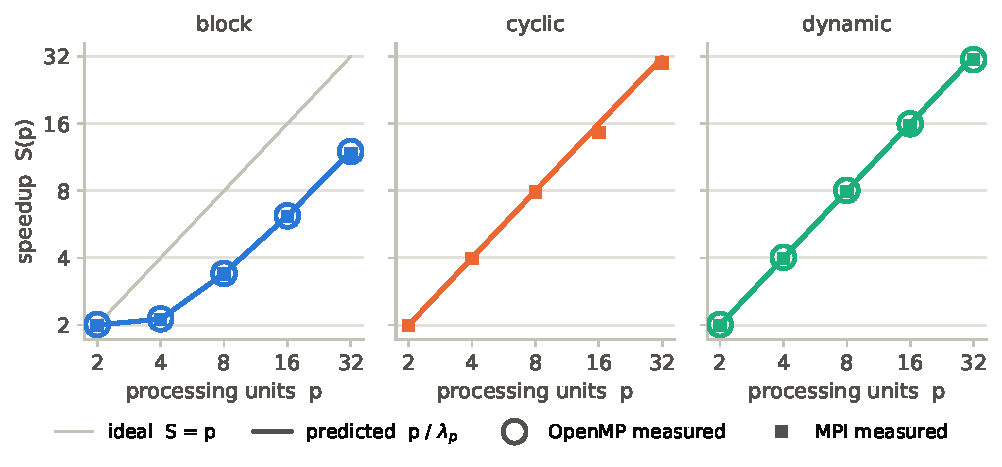
\includegraphics[width=\textwidth]{Immagini/grafici/cpu_predicted_vs_measured}
    \caption{Speedup misurato contro il limite $p/\lambda_p$ previsto dal profilo di
    carico seriale, un pannello per regola di assegnamento. La linea è il limite
    previsto, gli anelli le misure OpenMP, i quadrati le misure MPI; la retta
    grigia è l'ideale $S = p$. Assi logaritmici in base $2$; i dati sono quelli
    della tabella~\ref{tab:validazione-regole}.}
    \label{fig:cpu-predicted-measured}
\end{figure}

\paragraph{Lo statico satura il limite predetto.}
Per la regola a blocchi l'accordo con \texttt{schedule(static)} è entro lo
$0{,}6\%$ su tutti e cinque i punti. La decomposizione statica non lascia quindi
margine di ottimizzazione implementativa, perché tocca già il proprio limite
teorico: la perdita del $62\%$ di efficienza a $32$ thread non è imputabile a
overhead di OpenMP, a cache o a sincronizzazione, che insieme valgono meno dello
$0{,}6\%$, ma unicamente al fatto che le righe costose dell'insieme sono contigue
e finiscono nello stesso blocco. L'unica via per superarla è cambiare regola di
assegnamento.

\paragraph{La previsione dipende dalla regola, non dal paradigma.}
Il risultato che la tabella rende visibile è che la previsione dipende dalla
\emph{regola} e non dal meccanismo. Le due realizzazioni della regola a blocchi
--- una clausola \texttt{schedule(static)} in memoria condivisa e una
decomposizione esplicita con gather collettiva in memoria distribuita --- cadono
sullo stesso limite predetto entro pochi decimi di punto fino a $p=16$, pur non
avendo in comune né il modello di memoria né il lanciatore. Lo stesso vale per la regola dinamica, dove uno scheduler di runtime
e un protocollo master--worker esplicito arrivano a $30{,}99$ e $31{,}10$ su un
limite di $32{,}00$. Poiché $\lambda_p$ è calcolato dal solo $\{w_r\}$ seriale,
questa coincidenza è la conferma più solida del modello predittivo: la stessa riga di previsione governa due implementazioni indipendenti.

La regola ciclica, che lo sweep OpenMP non esercitava e che restava priva di
verifica, è ora confermata dove il modello è più esposto: prevede
$\lambda_p \approx 1$ e quindi speedup quasi ideale, e il cyclic lo raggiunge
entro l'$1\%$ fino a $p=8$. È la conferma che $\lambda_p$ non si limita a
descrivere un fallimento --- come faceva per i blocchi --- ma predice anche il
successo di una regola alternativa.

\paragraph{Dove il modello smette di predire, e perché.}
Tre scostamenti escono dal margine, e ciascuno indica un termine di costo che il
modello compute-only~\eqref{eq:makespan} per costruzione non contiene.

Il primo è la regola dinamica ai valori più alti di $p$: a $p=32$ entrambi i
meccanismi si fermano attorno al $97\%$ del limite ($-3{,}2\%$ OpenMP, $-2{,}8\%$
MPI). Il modello del makespan tratta il lavoro come frazionabile a piacere,
mentre l'unità indivisibile è la riga: l'ultima riga assegnata a un worker può
essere la più pesante, e questo \emph{effetto coda} riduce il limite di al più
$(\lambda_{\text{riga}} - 1)\,p/H$, cioè il $2{,}8\%$ a $p=16$ e il $5{,}5\%$ a
$p=32$. Tutte le misure dinamiche restano dentro questo margine. Per OpenMP vi
contribuisce anche la contesa sulla coda condivisa
(sezione~\ref{sec:openmp-risultati}), e i dati non permettono di separare i due
termini.

Il secondo è \texttt{cyclic} a $p=16$ e $p=32$ ($-8{,}5\%$ e $-5{,}8\%$), l'unico
caso in cui lo scarto è grande e non ha spiegazione dentro il modello: come
discusso nella sezione~\ref{sec:mpi-risultati}, la causa candidata è il riordino
seriale di de-interlacciamento su rank $0$, un costo di implementazione
indipendente da $p$ e quindi invisibile a una previsione fondata sul solo
profilo di carico, che però non spiega da solo lo scarto a $p=16$. Quel punto è
anche il più rumoroso della campagna e va rimisurato.

Il terzo è \texttt{block} MPI a $p=32$ ($-2{,}7\%$, contro il $-0{,}2\%$ della
realizzazione OpenMP della stessa regola). La gather ne spiega poco meno della
metà, pesando l'$1{,}2\%$ del tempo; il resto non è attribuibile con le misure
disponibili. Questi scostamenti corrispondono ai termini che il modello non
include --- granularità finita, costi di implementazione, comunicazione --- e
nessuno supera l'$8{,}5\%$ sui venticinque punti di misura.

\paragraph{Conseguenza interpretativa.}
Che le regole statiche saturino il proprio limite entro frazioni di punto
percentuale ha un effetto sulla lettura di tutto il lavoro: gli scostamenti
dallo speedup ideale qui osservati non originano da una frazione seriale nel
senso di Amdahl --- che nel codice è trascurabile --- ma dalla distribuzione del
lavoro. Vanno perciò letti attraverso $\lambda_p$ più che attraverso la metrica
di Karp--Flatt, che pure li segnala correttamente ma li attribuisce a una causa
che questo codice non ha: le forme chiuse di $e(p)$ ricavate per lo
\texttt{static} di OpenMP (sezione~\ref{sec:openmp-risultati}) e per il block
MPI (sezione~\ref{sec:mpi-risultati}) mostrano che la ``frazione seriale
sperimentale'' non è che $\lambda_p$ riscritto in un'altra variabile. È il
criterio con cui vanno lette tutte le colonne $e(p)$ di questo capitolo.

%-------------CUDA----------------------
\subsection{CUDA: acceleratore grafico}
\label{sec:cuda}
Con CUDA cambia il modello di esecuzione. Il pixel resta l'unità indipendente
(sezione~\ref{sec:parallelizzazione}), ma non viene più raggruppato in righe
distribuite fra poche unità di calcolo: ciascun pixel è affidato a uno dei
migliaia di thread della GPU.

L'hardware non esegue i thread singolarmente, ma li organizza in tre livelli. La
\emph{griglia} è l'insieme di tutti i \emph{blocchi}, ciascuno dei quali viene
assegnato per intero a uno Streaming Multiprocessor
(SM)~\cite{nvidia_ada_arch}. All'interno del blocco i thread sono numerati con la formula
$\texttt{id} = \texttt{threadIdx.x} + \texttt{threadIdx.y} \cdot
\texttt{blockDim.x}$, e l'SM li esegue in gruppi di $32$ id consecutivi ---
i \emph{warp}~\cite{nvidia_cuda_cc}. Ogni warp avanza con un unico program counter: i suoi $32$ thread
eseguono la stessa istruzione nello stesso ciclo secondo il modello SIMT
(Single Instruction, Multiple Threads). Il warp scheduler non conosce la
struttura 2D che si è dichiarata: vede solo id lineari e ne prende $32$ alla volta.

Questa linearizzazione è il punto critico per il problema in esame. Con
$\texttt{blockDim.x} = 32$, i thread $0$--$31$ hanno tutti
$\texttt{threadIdx.y} = 0$, cioè appartengono alla stessa riga del blocco; il
cambio di riga scatta solo all'id $32$, che è già nel warp successivo. Con
$\texttt{blockDim.x} = 16$, invece, il thread con $\texttt{id} = 16$ ha
$\texttt{threadIdx.x} = 0$, $\texttt{threadIdx.y} = 1$: il cambio di riga cade
a metà warp, e il warp $0$ finisce per contenere i pixel delle colonne $0$--$15$
della riga $0$ e delle colonne $0$--$15$ della riga $1$. In generale, per
$\texttt{blockDim.x}$ divisore di $32$, ogni warp copre $32/\texttt{blockDim.x}$
righe.

Quando un warp copre più righe si pongono due questioni distinte.
\begin{itemize}
    \item \textbf{Coalescenza.} La matrice è memorizzata in ordine row-major:
    pixel della stessa riga sono contigui in memoria, e $32$ scritture contigue
    possono essere servite in una sola transazione. Se il warp scrive su più
    righe gli indirizzi non sono più contigui e servono più transazioni, fino a
    $32$ volte il traffico per gli stessi dati.
    \item \textbf{Divergenza.} Le $32$ lane di un warp eseguono insieme, ma
    richiedono in generale un numero diverso di iterazioni: il warp termina solo
    quando termina la lane più lenta, e le lane già uscite consumano cicli con il
    risultato mascherato. Il costo del warp è quindi il massimo di $n_{i,j}$ sulle
    sue lane, invece della media, e la frazione di cicli sprecati è
    $1 - \overline{n}/\max n$. Un warp confinato in una riga non azzera la
    divergenza, perché una riga che attraversa il bordo contiene pixel interni ed
    esterni; un warp che riunisce righe diverse può però accostare situazioni
    ancora più eterogenee, per esempio pixel esterni in una riga e pixel di
    un'antenna nella riga successiva.
\end{itemize}
\vspace{3mm}
\begin{figure}[htbp]
    \centering
    \begin{subfigure}[t]{0.48\textwidth}
        \centering
        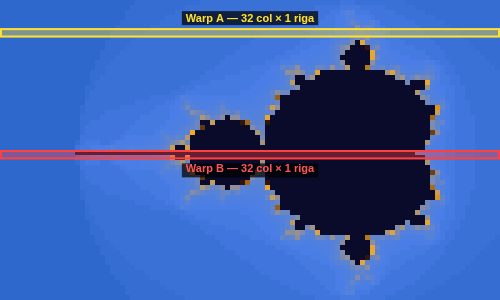
\includegraphics[width=\textwidth]{Immagini/warp_dim32}
        \caption{$\texttt{blockDim.x} = 32$: ogni warp occupa esattamente una riga.
        Il warp~A (giallo) cade in una zona esterna, dove tutti i pixel sfuggono in
        poche iterazioni; il warp~B (rosso) attraversa il bordo frattale, dove
        convivono pixel interni ed esterni con escape time molto diversi. Questa
        varianza dipende dalla geometria del problema, non dalla scelta del
        blocco.}
        \label{fig:warp-bdx32}
    \end{subfigure}
    \hfill
    \begin{subfigure}[t]{0.48\textwidth}
        \centering
        
\includegraphics[width=\textwidth]{Immagini/warp_dim16}
        \caption{$\texttt{blockDim.x} = 16$: ogni warp copre due righe (la linea
        tratteggiata segna il confine). Il warp~A resta omogeneo, perché entrambe
        le righe cadono in zona esterna; nel warp~B le due righe possono
        campionare strutture diverse del bordo, e la varianza degli escape time
        può crescere rispetto al caso a riga singola.}
        \label{fig:warp-bdx16}
    \end{subfigure}
    \caption{Mappatura dei warp sulla griglia degli escape time al variare di
    $\texttt{blockDim.x}$; la risoluzione dell'immagine e l'estensione dei warp
    sono illustrative. In entrambe le figure sono evidenziati un warp in zona
    esterna (A, giallo) e uno sul bordo frattale (B, rosso). L'ipotesi illustrata è
    che riunire più righe in un warp possa aumentare la divergenza, oltre a
    spezzare la coalescenza; la sezione~\ref{sec:cuda-previsioni} ne quantifica
    l'effetto medio sull'intera immagine.}
    \label{fig:warp-divergenza}
\end{figure}
\vspace{5mm}
Come mostra la figura~\ref{fig:warp-divergenza}, la scelta
$\texttt{blockDim.x} = 32$, o un suo multiplo, garantisce che i $32$ id
consecutivi di un warp stiano sempre sulla stessa riga: le scritture restano
coalescenti, ed è esclusa la divergenza aggiuntiva dovuta all'accostamento di
righe diverse. $\texttt{blockDim.y}$ resta libero, perché determina quante righe
gestisce il blocco ma non la forma dei warp. Per questo la scelta
$\texttt{threadIdx.x} \to$ colonna, $\texttt{threadIdx.y} \to$ riga non è una
convenzione neutra. Si tratta tuttavia di un'ipotesi da verificare: un blocco
compatto riunisce pixel vicini in entrambe le direzioni, e in media potrebbe
produrre warp non meno omogenei di una riga. Le previsioni della
sezione~\ref{sec:cuda-previsioni} e le misure della
sezione~\ref{sec:cuda-risultati} ne quantificano l'effetto.

La varianza per pixel degli escape time è la stessa irregolarità discussa fin
dall'inizio del lavoro, che si manifesta come sbilanciamento del carico sulla CPU
e come divergenza dei warp sulla GPU.

L'aritmetica del kernel è identica a quella seriale, in doppia precisione, e il
build impone \texttt{-{}-fmad=false}, l'analogo per \texttt{nvcc} di
\texttt{-ffp-contract=off}: la contrazione in fused multiply-add cambierebbe
l'ultimo bit e quindi $\pm 1$ iterazione sui pixel di bordo, rendendo il checksum
incomparabile con la baseline. La L40S dispone inoltre di tensor core, progettati
per le moltiplicazioni fra matrici dense~\cite{nvidia_ada_arch}: il kernel,
scalare e per pixel, non ne fa uso per costruzione.

% ============================================================
\subsubsection{Design dello sweep}
\label{sec:cuda-sweep}
% ============================================================

La domanda progettuale è la stessa delle sezioni precedenti: \emph{come} mappare
il lavoro sulle unità di calcolo, non \emph{quanto}. Sulla GPU la variabile di
controllo non è il numero di core --- fisso per la scheda --- ma la
\emph{geometria del blocco}, ovvero la forma $B_x \times B_y$ con cui i thread vengono
organizzati, e che determina simultaneamente la struttura dei warp, la
coalescenza degli accessi in memoria e l'occupancy degli SM. Lo sweep si articola
in due esperimenti ortogonali, ciascuno con la propria domanda.

\paragraph{Sweep A --- geometria del blocco.}
Vengono fissati i parametri del problema ($1024^2$, $N_{\max}=1000$, come in
tutti gli altri sweep), e si fa variare la sola forma del blocco su nove
geometrie appartenenti a quattro gruppi distinti. L'esperimento risponde alla
domanda: qual è la mappatura thread$\to$pixel migliore, e perché?
La maggior parte delle geometrie ha lo stesso numero totale di thread
per blocco ($256$); ciò che varia è la loro distribuzione su righe e colonne,
che determina la struttura dei warp e quindi coalescenza e divergenza. Le due
eccezioni, $512{\times}1$ e $128{\times}1$, servono a isolare l'effetto
del numero di thread a geometria del warp fissa.

\begin{itemize}
    \item \textbf{Warp orizzontali puri} ($256{\times}1$, $512{\times}1$,
    $128{\times}1$): $\texttt{blockDim.x}$ multiplo di $32$, scritture
    coalescenti. Variano la taglia del blocco, e con essa potenzialmente
    l'occupancy, a coalescenza e divergenza fisse: è il gruppo di riferimento.
    \item \textbf{Quadrati 2D coalescenti} ($128{\times}2$, $64{\times}4$,
    $32{\times}8$): con \texttt{blockDim.x} multiplo di $32$, ogni warp prende 32 id consecutivi che
    stanno tutti sulla stessa riga. Quindi la coalescenza è intatta e la
    divergenza è la stessa dei warp orizzontali puri.
    La differenza rispetto al primo gruppo è solo \texttt{blockDim.y}:
    cambia quanti warp risiedono in un SM, e con essi potenzialmente l'occupancy.
    Isola l'effetto di avere più righe per
    blocco.
    \item \textbf{Coalescenza violata} ($16{\times}16$, $8{\times}32$):
    $\texttt{blockDim.x} < 32$, ogni warp ripiega su più righe, spezzando gli
    accessi in memoria in più transazioni. Questo gruppo mette in luce un aspetto interessante
    dello sweep: un quadrato compatto come $16{\times}16$
    raggruppa pixel più vicini fra loro e potrebbe avere divergenza
    \emph{inferiore} a quella dei warp orizzontali (campionando una regione più
    stretta del piano), ma a prezzo di coalescenza violata. Divergenza e
    coalescenza tirano in direzioni opposte: non esiste una scelta vincente a priori, e solo il tempo
    di esecuzione può stabilire quale effetto prevalga.
    \item \textbf{Warp verticale} ($1{\times}256$): la configurazione prevede $32$ pixel della stessa
    colonna, tali che gli indirizzi sono distanti $W \cdot 4$ byte l'uno dall'altro. Si tratta pertanto del caso
    peggiore per la coalescenza. La divergenza, però, è quasi identica
    a quella dei warp orizzontali: non c'è nessuna direzione privilegiata in cui il problema sia ``più omogeneo'' e,
    di conseguenza, la varianza di $n$ tra due pixel
    adiacenti in orizzontale è comparabile a quella tra due pixel adiacenti in
    verticale. Questo rende $256{\times}1$ contro $1{\times}256$ l'esperimento più pulito dello sweep: divergenza simile,
    coalescenza opposta. La differenza di tempo misurata è quindi imputabile
    principalmente alla penalità di coalescenza.
\end{itemize}

Vale la pena chiarire perché $1{\times}256$ non è l'analogo GPU della
decomposizione ciclica MPI. Nel ciclico MPI il rank $r$ riceveva righe sparse
per l'intera immagine, mescolando righe leggere e pesanti; l'analogo GPU sarebbe
un warp i cui $32$ pixel sono prelevati da righe distanti anziché adiacenti.
Quella configurazione avrebbe divergenza massima e accessi non coalescenti, e
sarebbe il caso peggiore per entrambe le leve; non è realizzabile con una forma
di blocco, ma il suo costo si può stimare dalla matrice degli escape time
(sezione~\ref{sec:cuda-previsioni}). La $1{\times}256$, invece, rompe la
coalescenza ma lascia pressoché intatta la divergenza, ed è per questo un
controllo utile.

Il risultato atteso dallo Sweep A è la classifica delle nove geometrie per
$T_{\min}$, insieme alla verifica di quanto le grandezze calcolabili dalla sola
matrice degli escape time (sezione~\ref{sec:cuda-previsioni}) ne anticipino
l'ordinamento: è l'analogo di $\lambda_p$, che sul lato CPU prevedeva lo speedup
(sezione~\ref{sec:serial-pred-lambdaP}).

\paragraph{Sweep B --- saturazione e trasferimento.}
Viene fissata la forma del blocco $256{\times}1$, riferimento a warp
orizzontali, e si fanno variare i valori dei parametri del problema. Sulla GPU
non è infatti il numero di core a variare, bensì il loro \emph{utilizzo}. La
scalabilità della GPU non è quindi una curva su $p$ come per OpenMP e MPI,
ma è una curva di \emph{saturazione}: al crescere della taglia del problema
cresce il numero di warp lanciati, e con essi l'occupazione degli SM, e le prestazioni in GFLOP/s, fino al
punto in cui aggiungere pixel non produce più guadagno proporzionale. Oltre
quella soglia la scheda è sfruttata appieno. Lo sweep si compone di due
esperimenti.

\textbf{B1 -- saturazione}: risoluzione $512^2 \to 1024^2 \to 2048^2 \to
4096^2$ a $N_{\max}=1000$ fisso.
Al crescere della risoluzione aumenta il
numero di warp lanciati e con essi l'occupazione degli SM: la curva di
throughput effettivo in GFLOP/s dovrebbe salire e appiattirsi verso il picco.
La domanda è \textit{da quale taglia} la scheda è sfruttata appieno, e quale
fattore la penalizza sotto quella soglia: overhead di lancio del kernel,
trasferimento incomprimibile o SM non saturi.

\textbf{B2 -- trasferimento}: $N_{\max} \in \{500, 1000, 5000\}$ a risoluzione
$2048^2$ fissa.
A pixel fissi i byte da copiare sono costanti, mentre il
calcolo cresce con $N_{\max}$: ci si attende che la frazione
$\texttt{transfer\_time}/T$ cali, mostrando l'ammortamento del costo di copia,
i cui contributi sono descritti nella sezione~\ref{sec:cuda-metriche}, al
crescere del lavoro. È il termine ``alla Amdahl'' del percorso
host$\leftrightarrow$device, e la curva B2 lo quantifica.

Ogni punto di B lancia il seriale e la GPU sullo stesso nodo nella stessa
esecuzione, così $S = T(1)/T_{\text{gpu}}$ è same-hardware per costruzione: un
core CPU contro una GPU, con la baseline seriale rigenerata a ogni confronto. Il
punto a $1024^2$ e $N_{\max}=1000$ ripete la configurazione $256{\times}1$ dello
Sweep~A con lo stesso numero di ripetizioni, e fa quindi da controllo fra i due
job.

% ============================================================
\subsubsection{Metriche specifiche}
\label{sec:cuda-metriche}
% ============================================================

Sulla GPU il numero di core è fissato dalla scheda e non è una variabile
controllabile: al crescere del problema cresce la loro occupazione, non il loro
numero. Il parametro $p$ è quindi degenere, e con esso efficienza e metrica di
Karp--Flatt, che presuppongono un numero variabile di unità di calcolo. Lo
speedup è definito come $S = T_1/T_{\text{gpu}}$, dove $T_1$ è il tempo della
baseline seriale su un core della CPU dello stesso nodo: è il confronto fra due
implementazioni dello stesso problema, non fra configurazioni a $p$ variabile.

Tre grandezze sono proprie di questo paradigma.

La \textbf{divergenza} è misurata tramite un proxy deterministico calcolato
dalla matrice degli escape time: per ogni gruppo di $32$ pixel contigui secondo
la mappatura del kernel, si calcola la varianza dei valori $n_{i,j}$; la media
di queste varianze su tutti i gruppi è il proxy. Poiché l'unico branch del
kernel è il ciclo di escape, la divergenza dipende soltanto dagli escape time dei
pixel riuniti nel warp, ed è quindi interamente calcolabile dalla matrice. Questo approccio è preferibile alla misura
strumentata con un profiler per tre ragioni: è deterministico e privo di rumore,
non richiede permessi sui performance counter (spesso non disponibili sui
cluster), e non perturba i tempi di esecuzione.

L'\textbf{occupancy} è teorica e si ottiene dall'API runtime. In linea di
principio il suo valore dipende dal numero di registri che il kernel impiega per
thread, riportato da \texttt{-Xptxas -v}: il kernel mantiene attive più
variabili in doppia precisione ($z_{\text{real}}$, $z_{\text{imag}}$, i
rispettivi quadrati, $c_{\text{real}}$ e $c_{\text{imag}}$), e registri
insufficienti limiterebbero i warp che possono risiedere contemporaneamente su un
SM. Un'occupancy elevata non implica tuttavia prestazioni migliori: serve a
mascherare le latenze di memoria, mentre il kernel è limitato dal calcolo, con
fino a $8\,N_{\max}$ FLOP per ogni scrittura da $4$ byte. La leva attesa come
primaria è quindi la divergenza.

Il \textbf{tempo di trasferimento} device$\to$host è misurato con CUDA event
attorno alla copia della matrice risultante ($4$ byte per pixel). Non esiste
traffico host$\to$device: gli input del kernel sono scalari passati come
argomenti al lancio, senza alcuna \texttt{cudaMemcpy}.
Poiché il costo di copia è fisso in byte mentre il calcolo cresce con
$N_{\max}$, la grandezza di interesse è la frazione $\texttt{transfer\_time}/T$, che è attesa calare
all'aumentare di $N_{\max}$: lo Sweep~B2 quantifica questo ammortamento.

\paragraph{Che cosa comprende il tempo di trasferimento.}
La copia della matrice dalla GPU alla memoria del processo non è un'unica
operazione: il tempo misurato somma tre contributi,
\[
    T_{\text{transfer}} = T_{\text{PCIe}} + T_{\text{socket}} + T_{\text{host}}.
\]
\begin{itemize}
    \item $T_{\text{PCIe}}$ è il trasferimento sul bus della scheda, un
    collegamento PCIe~4.0~x16 con una banda nominale di circa $31{,}5$~GB/s per
    direzione;
    \item $T_{\text{socket}}$ è l'eventuale attraversamento
    dell'interconnessione fra i due socket del nodo, nullo quando il processo
    gira sul socket a cui è collegata la GPU;
    \item $T_{\text{host}}$ è la copia in memoria host: la matrice risiede in
    memoria ordinaria, che la GPU non può scrivere direttamente, per cui il
    driver trasferisce i dati in un buffer intermedio e li copia poi nella
    destinazione.
\end{itemize}

Il termine centrale dipende da una scelta che non è sotto il controllo del job.
Il nodo è dual-socket (sezione~\ref{sec:ambiente}), e ciascuna delle otto GPU è
collegata a uno dei due socket; in assenza di richieste esplicite, SLURM assegna
la GPU e il core del processo in base alla disponibilità del momento. Da un job
all'altro il processo può quindi trovarsi sullo stesso socket della GPU, il caso
locale, oppure sull'altro, il caso cross-NUMA (figura~\ref{fig:numa-topology}).
Poiché \texttt{nvidia-smi} non riporta l'affinità NUMA della scheda, il job dello
Sweep~B la ricava da \texttt{sysfs} e registra nel log sia il socket del
processo sia i core locali alla GPU
(\repofile{mandelbrot/job_sbatch/mandel_cuda_scaling.sh}). Ogni valore di
\texttt{transfer\_time} viene così letto rispetto al posizionamento effettivo del
proprio job, e non rispetto a uno presunto.
\vspace{2,5mm}
\begin{figure}[htbp]
    \centering
    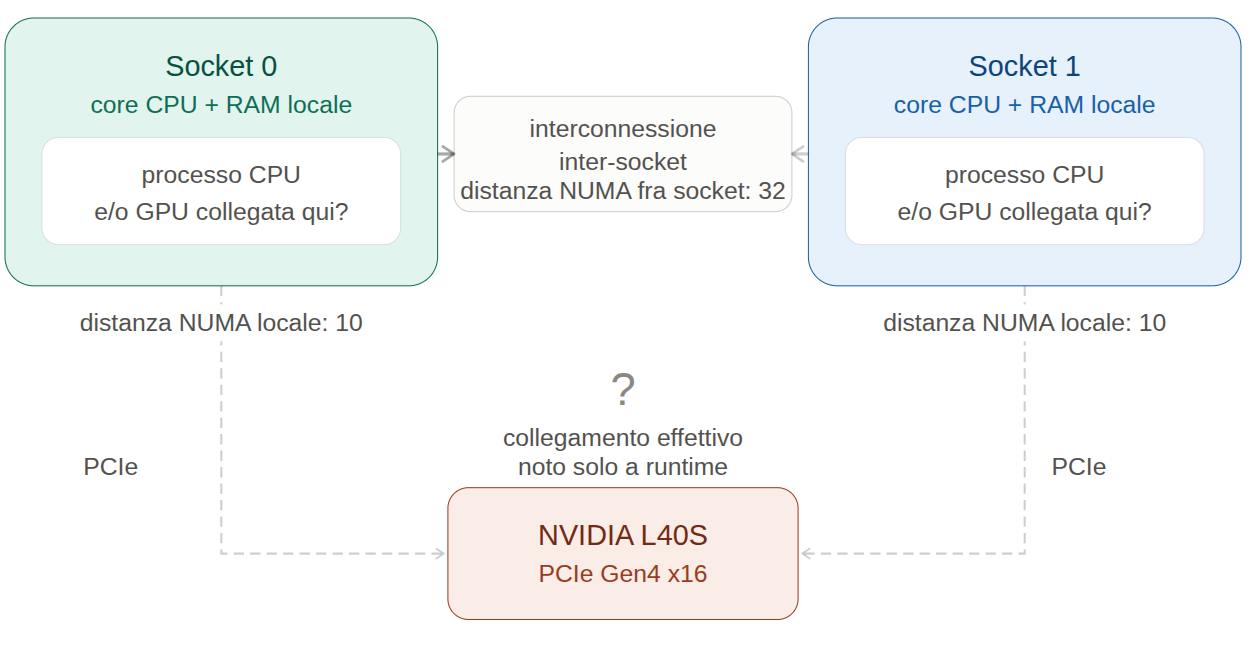
\includegraphics[width=0.8\textwidth]{Immagini/numa_topology}
    \caption{Topologia NUMA di \texttt{gnode01}. Ciascun socket dispone dei
    propri core e della propria memoria locale; i due socket sono collegati da
    un'interconnessione, per la quale il firmware dichiara una distanza NUMA di
    $32$ contro $10$ dell'accesso locale, un valore relativo e non una misura di
    latenza. La GPU è collegata tramite PCIe a uno dei due socket, e il processo
    può essere eseguito sullo stesso socket o sull'altro: nel secondo caso la
    copia della matrice attraversa anche l'interconnessione.}
    \label{fig:numa-topology}
\end{figure}

% ============================================================
\subsubsection{Frammenti di codice rilevanti}
\label{sec:cuda-codice}
% ============================================================

Nei due paradigmi precedenti il kernel seriale restava riconoscibile: OpenMP vi
anteponeva una direttiva, MPI lo racchiudeva in un protocollo di messaggi. Con
CUDA scompaiono invece i due cicli annidati sui pixel: ogni thread esegue una
sola volta il corpo del ciclo e deve ricavare autonomamente il pixel di propria
competenza. La ricorrenza di escape è identica a quella seriale e non viene
riportata; il codice completo è in \repofile{mandelbrot/src/mandelbrot_cuda.cu}.

\begin{verbatim}
__global__ void mandelbrot_kernel(int* escape_counts, int width, int rows,
                                  Viewport view, double dx, double dy,
                                  int max_iter) {
    const int col = blockIdx.x * blockDim.x + threadIdx.x;
    const int row = blockIdx.y * blockDim.y + threadIdx.y;
    if (col >= width || row >= rows) return;     // lanes beyond the image

    // c_real, c_imag: centre of pixel (row, col), as in the serial kernel
    escape_counts[row * width + col] = escape_time(c_real, c_imag, max_iter);
}
\end{verbatim}

Le variabili \texttt{col} e \texttt{row} realizzano l'intera assegnazione del
lavoro. Ogni thread dispone di tre terne predefinite: \texttt{threadIdx}, la
posizione del thread all'interno del proprio blocco, con componenti comprese fra
$0$ e $\texttt{blockDim}-1$; \texttt{blockIdx}, la posizione del blocco
all'interno della griglia; \texttt{blockDim}, le dimensioni del blocco. Lungo
ciascun asse il prodotto $\texttt{blockIdx}\cdot\texttt{blockDim}$ è il numero di
thread contenuti nei blocchi che precedono quello corrente, e coincide quindi con
la coordinata del primo pixel del blocco; sommandovi \texttt{threadIdx} si ottiene
la coordinata globale del thread. \texttt{col} è pertanto l'indice di colonna del
pixel e \texttt{row} il suo indice di riga (\texttt{rows} coincide con l'altezza
dell'immagine quando la simmetria non è attiva): la coppia individua l'unica cella
della matrice degli escape time che il thread calcola e scrive. L'associazione
dell'asse $x$ alle colonne è la scelta motivata nella sezione~\ref{sec:cuda}. Come
l'indice di riga globale dei rank MPI (sezione~\ref{sec:mpi-codice}), il compito
non viene comunicato al thread ma ricavato dalla sua posizione; a differenza di
MPI, l'unità assegnata non è una riga ma un singolo pixel.

La guardia successiva è necessaria perché la griglia è dimensionata per eccesso
(frammento seguente): quando le dimensioni dell'immagine non sono multiple di
quelle del blocco, i blocchi dell'ultima riga o colonna della griglia si
estendono oltre l'immagine, e i thread corrispondenti devono terminare senza
scrivere. Si osservi infine che nessuna istruzione del kernel dipende dalla forma
del blocco: le nove geometrie dello Sweep~A eseguono lo stesso codice e
differiscono soltanto per l'insieme di pixel che condividono un warp.

\begin{verbatim}
static const dim3 block = block_shape_from_env();       // MANDEL_BLOCK=BXxBY
static const double occupancy = launch_occupancy(block);
const dim3 grid((width + block.x - 1) / block.x,          // ceiling division
                (computed_rows + block.y - 1) / block.y);
mandelbrot_kernel<<<grid, block>>>(d_escape_counts, width, computed_rows, ...);
\end{verbatim}

La forma del blocco è letta a esecuzione dalla variabile d'ambiente
\texttt{MANDEL\_BLOCK}, analogamente a quanto avviene con la variabile
\texttt{OMP\_SCHEDULE} per OpenMP e con la variabile \texttt{MPI\_DECOMP} per
MPI: un solo eseguibile copre così tutte le geometrie dello sweep. Forma del blocco e occupancy, che dipende soltanto da essa, sono
determinate una volta per processo (\texttt{static}); la griglia è invece
ricalcolata a ogni chiamata, poiché dipende dalla risoluzione, che lo Sweep~B fa
variare.

Il frammento più rilevante per l'analisi non appartiene al kernel, ma al codice
condiviso delle metriche (\repofile{mandelbrot/src/metrics.cpp}), che calcola
divergenza e spreco sulla matrice degli escape time. Per
ogni blocco della griglia, di indici \texttt{bx} e \texttt{by}, i thread vengono
raggruppati in warp di $32$ id consecutivi e ciascun id viene ricondotto al
proprio pixel:

\begin{verbatim}
for (long long start = 0; start < threads_per_block; start += warp_size) {
    lane.clear();                            // lanes of one warp
    const long long end = std::min(start + warp_size, threads_per_block);
    for (long long id = start; id < end; ++id) {
        const int col = bx * block_x + static_cast<int>(id % block_x);
        const int row = by * block_y + static_cast<int>(id / block_x);
        if (col < width && row < height)
            lane.push_back(img.data[row * width + col]);
    }
    // accumulate var(lane) and 1 - mean(lane) / max(lane)
}
\end{verbatim}

Le espressioni di \texttt{col} e \texttt{row} sono quelle del kernel, con la
posizione del thread nel blocco ricavata dall'id lineare invertendo la formula
della sezione~\ref{sec:cuda}: $\texttt{threadIdx.x} = \texttt{id} \bmod
\texttt{blockDim.x}$ e $\texttt{threadIdx.y} = \lfloor \texttt{id} /
\texttt{blockDim.x} \rfloor$. Il raggruppamento riproduce quindi esattamente
quello operato dal warp scheduler, ed è per questo che divergenza e spreco sono
previsioni disponibili prima dell'esecuzione del kernel. Le lane che cadono oltre
l'immagine sono escluse, affinché entrambe le grandezze misurino la variabilità
indotta dal frattale e non gli effetti di bordo della suddivisione in blocchi.
Coerentemente con il contratto delle metriche, il calcolo risiede nel driver
condiviso e non nel kernel.

Due ulteriori accorgimenti allineano la regione misurata al contratto comune agli
altri paradigmi (allocazione inclusa, I/O escluso):

\begin{verbatim}
const ContextInit g_context_init;   // ctor: cudaFree(nullptr) -> context

cudaEventRecord(before_copy);       // queued behind the kernel, same stream
cudaMemcpy(img.data.data(), d_escape_counts, bytes, cudaMemcpyDeviceToHost);
cudaEventRecord(after_copy);        // elapsed(before, after) = pure D2H
\end{verbatim}

Il primo riguarda il contesto CUDA, la cui creazione, eseguita alla prima
chiamata all'API, richiede centinaia di millisecondi: l'oggetto statico
\texttt{g\_context\_init} lo crea prima dell'avvio del cronometro, così che il
costo non ricada sulla prima ripetizione. Il secondo riguarda il tempo di
trasferimento: i due event sono accodati sullo stesso stream del kernel, che
esegue le operazioni in ordine, quindi \texttt{before\_copy} viene raggiunto solo
al termine del kernel e l'intervallo misurato comprende la sola copia
device$\to$host.

Le grandezze proprie della GPU raggiungono il CSV attraverso accessori dichiarati
nell'header comune (\texttt{kernel\_occupancy()},
\texttt{kernel\_transfer\_seconds()} e le dimensioni del blocco), che i kernel
CPU definiscono nulli: il medesimo driver produce così lo stesso schema di record
per tutti i paradigmi.

% ============================================================
\subsubsection{Previsioni dalla matrice degli escape time}
\label{sec:cuda-previsioni}
% ============================================================

% Fonte: data/block_geometry.csv (analysis/block_geometry.py su
% figure_nmax1000.raw, matrice nuda 1024^2, N_max=1000, W = 259655490);
% divergenza e spreco coincidono con cuda_log_notes_34335.txt. Registri per
% thread dal log di build (-Xptxas -v).

Come per le decomposizioni CPU (sezione~\ref{sec:serial-pred-lambdaP}), il costo
delle geometrie del blocco può essere stimato prima di eseguire il kernel. La
forma del blocco determina quali pixel condividono un warp, e questo
raggruppamento è riproducibile sulla matrice degli escape time del baseline con
l'attraversamento della sezione~\ref{sec:cuda-codice}. Divergenza e spreco sono
calcolati anche dal binario CUDA durante lo sweep; cicli e costo dei blocchi sono
stati ricavati successivamente dalla stessa matrice, con
\repofile{mandelbrot/analysis/block_geometry.py}. In entrambi i casi le grandezze
dipendono dai soli dati seriali, ed è in questo senso che costituiscono
previsioni a priori.

Per ciascuna geometria si considerano quattro grandezze:
\begin{itemize}
    \item la \textbf{divergenza} e lo \textbf{spreco medio}, definiti
    rispettivamente nelle sezioni~\ref{sec:cuda-metriche} e~\ref{sec:cuda};
    \item i \textbf{cicli relativi}: poiché un warp termina solo quando termina
    la sua lane più lenta, i cicli eseguiti con una geometria sono
    $\sum_{\text{warp}} \ell \cdot \max n_{i,j}$, con $\ell$ numero di lane del
    warp; il loro rapporto con quelli della $256{\times}1$ è il tempo relativo
    previsto nell'ipotesi che il tempo sia proporzionale ai cicli;
    \item il \textbf{CoV del costo dei blocchi}, coefficiente di variazione dei
    cicli eseguiti per blocco, che descrive la granularità con cui il lavoro è
    suddiviso.
\end{itemize}
Non si riporta invece il rapporto fra costo massimo e costo medio dei blocchi,
che sarebbe l'analogo di $\lambda_p$: non appena un blocco cade interamente
all'interno dell'insieme, il suo costo è $N_{\max}$ per lane, e il rapporto si
riduce a $N_{\max}$ diviso i cicli medi per pixel ($1000/286{,}4 = 3{,}49$ per
tutte le geometrie orizzontali), senza alcuna informazione sulla forma del
blocco.
\vspace{2,5mm}
\begin{table}[htbp]
    \centering
    \begin{tabular}{lrrrrr}
        \hline
        Blocco & divergenza & spreco medio & cicli relativi & CoV blocchi & occ. \\
        \hline
        $128{\times}1$ & $10\,215$ & $11{,}24\%$ & $1{,}000$ & $1{,}41$ & $1{,}00$ \\
        $256{\times}1$ & $10\,215$ & $11{,}24\%$ & $1{,}000$ & $1{,}34$ & $1{,}00$ \\
        $512{\times}1$ & $10\,215$ & $11{,}24\%$ & $1{,}000$ & $1{,}25$ & $1{,}00$ \\
        $128{\times}2$ & $10\,215$ & $11{,}24\%$ & $1{,}000$ & $1{,}41$ & $1{,}00$ \\
        $64{\times}4$  & $10\,215$ & $11{,}24\%$ & $1{,}000$ & $1{,}51$ & $1{,}00$ \\
        $32{\times}8$  & $10\,215$ & $11{,}24\%$ & $1{,}000$ & $1{,}54$ & $1{,}00$ \\
        \hline
        $16{\times}16$ & $5\,932$  & $7{,}82\%$  & $0{,}947$ & $1{,}59$ & $1{,}00$ \\
        $8{\times}32$  & $3\,689$  & $6{,}23\%$  & $0{,}928$ & $1{,}59$ & $1{,}00$ \\
        \hline
        $1{\times}256$ & $9\,550$  & $11{,}75\%$ & $0{,}998$ & $1{,}33$ & $1{,}00$ \\
        \hline
        sparso         & $131\,050$ & $66{,}31\%$ & $2{,}501$ & --- & --- \\
        \hline
    \end{tabular}
    \caption{Previsioni per le geometrie dello Sweep~A, calcolate dalla sola
    matrice degli escape time del baseline ($1024^2$, $N_{\max}=1000$, kernel
    \emph{bare}) e, per l'occupancy, dall'API runtime. Le righe sono raggruppate
    per partizione in warp: orizzontale, compatta, verticale e sparsa. I cicli
    sono relativi alla $256{\times}1$. Il raggruppamento sparso non è realizzabile
    con una forma di blocco.}
    \label{tab:cuda-previsioni}
\end{table}

\paragraph{Quattro partizioni in nove geometrie.}
Il proxy vale $10\,215$ per tutte le sei geometrie con $\texttt{blockDim.x}$
multiplo di $32$. In questo caso, all'interno di ogni warp,
$\texttt{id} \bmod \texttt{blockDim.x}$ assume $32$ valori consecutivi e
$\lfloor \texttt{id}/\texttt{blockDim.x} \rfloor$ resta costante: il warp è
formato da $32$ pixel contigui della stessa riga, e ogni riga risulta suddivisa
in segmenti di $32$ pixel indipendentemente da $\texttt{blockDim.y}$. La
partizione in warp è quindi la stessa, e con essa divergenza, spreco e cicli; le
sei forme differiscono soltanto per la granularità dei blocchi, come mostra la
colonna del CoV. Le nove geometrie realizzano pertanto quattro partizioni
distinte. Le due compatte, $8{\times}32$ e $16{\times}16$, riuniscono pixel più
vicini nel piano e riducono i cicli del $7{,}2\%$ e del $5{,}3\%$; quella
verticale, $1{\times}256$, è quasi equivalente all'orizzontale ($-0{,}24\%$). Fra
le forme realizzabili il modello attribuisce dunque alla geometria del blocco un
peso di pochi punti percentuali. In media, inoltre, la matrice non conferma che
riunire righe diverse aumenti la divergenza: le partizioni compatte la riducono. I
casi locali di forte eterogeneità illustrati nella
figura~\ref{fig:warp-divergenza} restano possibili, ma pesano poco sulla media
dell'intera immagine.

\paragraph{Occupancy.}
L'occupancy prevista vale $1{,}00$ per tutte le geometrie. Il kernel impiega $22$
registri per thread, secondo il log di compilazione. Per la compute
capability~$8.9$ un SM dispone di $64$\,K registri e ospita al più $1\,536$
thread residenti, cioè $48$ warp da $32$ thread~\cite{nvidia_cuda_cc}: i
registri basterebbero per circa $90$ warp, ben oltre il limite, per cui il
vincolo effettivo è il numero di thread e non la disponibilità di registri. Tutte le geometrie usano inoltre
blocchi da $128$, $256$ o $512$ thread, divisori dei $1\,536$ thread di un SM,
che viene così riempito senza posti residui. L'occupancy non può dunque
distinguere le geometrie, e l'ipotesi della sezione~\ref{sec:cuda-metriche},
secondo cui il numero di variabili del kernel FP64 ne avrebbe limitato il valore,
è smentita già prima dell'esecuzione.

\paragraph{Il raggruppamento sparso.}
Nella forma calcolata, il pixel $p$ della matrice linearizzata è assegnato al
warp $p \bmod 32\,768$: ogni warp contiene $32$ pixel della stessa colonna, a
$32$ righe di distanza l'uno dall'altro, e campiona quindi l'intera altezza
dell'immagine. Il proxy vale $131\,050$, $12{,}8$ volte quello della partizione
orizzontale, lo spreco medio sale al $66\%$ e i cicli a $2{,}5$ volte: è il caso
peggiore anticipato nella sezione~\ref{sec:cuda-sweep}.

% ============================================================
\subsubsection{Analisi dei risultati}
\label{sec:cuda-risultati}
% ============================================================

% Dati Sweep A: job 34334 (--repeat 10) e 34335 (--repeat 30) su gnode01,
% partizione only-one-gpu, L40S, entrambi COMPLETED 0:0. Fonti: run_34334.csv,
% run_34335.csv e le note cuda_log_notes_*.txt, che conservano warp_div_scat,
% warp_wasted e i registri/thread: figure assenti dal CSV e presenti solo nel
% log di job, che non e' versionato.
%
% Previsioni: sec:cuda-previsioni (data/block_geometry.csv).
%
% Dati Sweep B: job 34424 su gnode01, partizione only-one-gpu, L40S diversa da
% quella dello Sweep A (UUID GPU-a554e585...), 30 ripetizioni GPU e 3 seriali.
% Fonti: run_34424.csv e cuda_log_notes_34424.txt, che conserva il
% posizionamento NUMA (GPU sul nodo 0, processo sul core 42 del socket 1).
% Regressioni (tempo di copia sui byte; T = c + tau*W nel B2) calcolate dai
% valori del CSV.

\paragraph{Sweep A -- geometria del blocco.}
La tabella~\ref{tab:cuda-blocks} riporta le nove geometrie, misurate in due
campagne distinte; tutte producono lo stesso checksum della baseline seriale.
Fra la più veloce ($1{\times}256$, $5{,}631$~ms) e la più lenta ($64{\times}4$,
$6{,}091$~ms) il divario è dell'$8{,}2\%$: su questo kernel la geometria del
blocco è una leva di second'ordine. I paragrafi seguenti verificano che il
divario sia sistematico, lo confrontano con le previsioni della
sezione~\ref{sec:cuda-previsioni} (occupancy e cicli) ed esaminano infine i due
effetti che la tabella delle previsioni non contiene: coalescenza e granularità
dei blocchi.
\vspace{2,5mm}
\begin{table}[htbp]
    \centering
    \caption{Sweep~A: tempi misurati per le nove geometrie del blocco ($1024^2$,
        $N_{\max}=1000$, kernel \emph{bare}), nello stesso ordine della
        tabella~\ref{tab:cuda-previsioni}. Le due colonne di tempo corrispondono ai
        job $34334$ ($10$ ripetizioni) e $34335$ ($30$ ripetizioni), entrambi su
        \texttt{gnode01}, partizione \texttt{only-one-gpu}. Il tempo relativo è
        riferito alla $256{\times}1$ nella campagna a $30$ ripetizioni e va letto
        contro i cicli relativi previsti; lo speedup è riferito alla baseline
        seriale del job $34335$, $T(1) = 0{,}720255$~s.}
    \label{tab:cuda-blocks}
    \begin{tabular}{lrrrr}
        \hline
        Blocco & $T_{\min}^{(10)}$ [ms] & $T_{\min}^{(30)}$ [ms] & $T/T_{256\times1}$ & $S$ \\
        \hline
        $128{\times}1$ & $5{,}802$ & $5{,}690$ & $0{,}985$ & $126{,}6$ \\
        $256{\times}1$ & $5{,}814$ & $5{,}776$ & $1{,}000$ & $124{,}7$ \\
        $512{\times}1$ & $6{,}057$ & $5{,}988$ & $1{,}037$ & $120{,}3$ \\
        $128{\times}2$ & $5{,}984$ & $5{,}957$ & $1{,}031$ & $120{,}9$ \\
        $64{\times}4$  & $6{,}244$ & $6{,}091$ & $1{,}055$ & $118{,}2$ \\
        $32{\times}8$  & $6{,}116$ & $6{,}086$ & $1{,}054$ & $118{,}3$ \\
        \hline
        $16{\times}16$ & $5{,}877$ & $5{,}860$ & $1{,}015$ & $122{,}9$ \\
        $8{\times}32$  & $5{,}865$ & $5{,}752$ & $0{,}996$ & $125{,}2$ \\
        \hline
        $1{\times}256$ & $5{,}623$ & $\mathbf{5{,}631}$ & $0{,}975$ & $127{,}9$ \\
        \hline
    \end{tabular}
\end{table}

\paragraph{Riproducibilità della classifica.}
Sei delle nove geometrie hanno $\texttt{blockDim.x}$ multiplo di $32$ e, come mostrato
nella sezione~\ref{sec:cuda-previsioni}, suddividono l'immagine negli stessi warp: divergenza, spreco e
occupancy coincidono, e nessuna di queste grandezze le distingue. Nella campagna
a $10$ ripetizioni i loro tempi minimi coprivano tuttavia un intervallo del
$7{,}6\%$, più del doppio del vantaggio della $1{\times}256$ sulla $256{\times}1$
($3{,}4\%$). Con una dispersione di tale ampiezza fra configurazioni equivalenti
rispetto ai predittori, non era possibile stabilire se la classifica fosse
riproducibile. La campagna a $30$ ripetizioni risolve la questione: l'ordinamento
si ripete con un solo scambio, fra la terza e la quarta posizione ($8{\times}32$
e $256{\times}1$, distanti lo $0{,}4\%$); nessun tempo minimo varia di più del
$2{,}5\%$ fra le due campagne, e quello della $1{\times}256$ varia dello
$0{,}14\%$. Le differenze sono quindi sistematiche e richiedono una spiegazione.

La stessa campagna conferma la scelta di $T_{\min}$ come statistica di
riferimento. Per la $8{\times}32$ si ha $T_{\text{mean}} = 11{,}21$~ms a fronte
di $T_{\text{median}} = 6{,}05$~ms: la mediana, allineata a quella delle altre
geometrie, esclude un rallentamento dell'intera serie, mentre lo scarto della
media corrisponde a un ritardo cumulato di circa $155$~ms sulle $30$ ripetizioni,
compatibile con una singola esecuzione disturbata da un evento esterno. Il minimo
non ne risente.

\paragraph{Occupancy.}
L'occupancy rilevata vale $1{,}00$ per tutte le geometrie, come previsto nella
sezione~\ref{sec:cuda-previsioni}, e non può quindi spiegare le differenze di tempo.

\paragraph{Cicli previsti e tempi misurati.}
La tabella~\ref{tab:cuda-previsioni} attribuisce alle partizioni compatte una
riduzione dei cicli del $7{,}2\%$ ($8{\times}32$) e del $5{,}3\%$ ($16{\times}16$)
rispetto alla $256{\times}1$. Se il tempo fosse determinato dai cicli dei warp, le
due geometrie dovrebbero risultare più veloci in misura analoga. La
tabella~\ref{tab:cuda-blocks} non lo conferma: la $8{\times}32$ guadagna lo
$0{,}4\%$ e la $16{\times}16$ è più lenta dell'$1{,}5\%$.

La previsione non è per questo errata: i cicli sono un calcolo esatto sulla
matrice e quantificano correttamente il lavoro mascherato. Ciò che la misura
smentisce è
l'ipotesi, formulata nella sezione~\ref{sec:cuda-metriche}, che tale lavoro sia la
leva primaria del tempo di esecuzione: nell'intervallo esplorato, riduzioni dei
cicli dei warp fino al $7\%$ non producono guadagni apprezzabili. Individuare la
componente che domina il tempo richiederebbe una misura strumentata, non
disponibile su questo cluster (si veda oltre).

\paragraph{Coalescenza.}
Il confronto fra $256{\times}1$ e $1{\times}256$ era stato progettato per isolare
la penalità di coalescenza. Le due geometrie hanno divergenza simile ($10\,215$ e
$9\,550$) e, secondo la tabella~\ref{tab:cuda-previsioni}, un numero di cicli dei warp che
differisce dello $0{,}24\%$; la prima scrive però $32$ indirizzi contigui per
warp, la seconda $32$ indirizzi distanti $4\,096$ byte l'uno dall'altro. In
presenza di una penalità di coalescenza la $1{\times}256$ risulterebbe più lenta;
la misura la indica invece più veloce del $2{,}5\%$ ($3{,}4\%$ nella campagna a
$10$ ripetizioni).

L'assenza di penalità si spiega confrontando il traffico di memoria con la banda
disponibile. Il kernel scrive $4$~MiB per lancio in $5{,}63$~ms, pari a circa
$0{,}74$~GB/s, a fronte degli $864$~GB/s di banda di memoria della
scheda~\cite{nvidia_ada_arch}. Anche
ammettendo che la perdita di coalescenza moltiplichi il traffico per il fattore
massimo di $32$ (sezione~\ref{sec:cuda}), si otterrebbero circa $24$~GB/s, meno
del $3\%$ della banda. In nessuna delle due configurazioni il canale di memoria si
avvicina alla saturazione, e il numero di transazioni non incide quindi sul tempo.
Il risultato costituisce la verifica sperimentale di quanto la
sezione~\ref{sec:cuda-metriche} aveva argomentato per via teorica: il kernel è
limitato dal calcolo e non dalla banda.

\paragraph{Granularità dei blocchi.}
Fra le tre geometrie orizzontali pure, che condividono partizione in warp,
divergenza, spreco e occupancy, il tempo cresce con la dimensione del blocco in
entrambe le campagne: $128{\times}1$ ($8\,192$ blocchi da $4$ warp,
$5{,}690$~ms), $256{\times}1$ ($4\,096$ blocchi da $8$ warp, $5{,}776$~ms),
$512{\times}1$ ($2\,048$ blocchi da $16$ warp, $5{,}988$~ms). Poiché l'unica
grandezza che varia è il numero di blocchi, la differenza del $5\%$ va attribuita
alla granularità con cui il lavoro viene distribuito sui $142$ SM del
chip~\cite{nvidia_ada_arch}.
L'interpretazione coerente con i dati è che blocchi più piccoli consentano di
ripartire il carico fra gli SM in modo più uniforme, avvicinando il completamento
dell'ultimo SM a quello medio. Ciò vale nonostante i blocchi più piccoli abbiano,
singolarmente, un costo più variabile (CoV $1{,}41$ contro $1{,}25$): è il loro
numero maggiore per SM a mediare il carico. Si tratta dello stesso meccanismo osservato con il
chunk in OpenMP (sezione~\ref{sec:openmp-risultati}), dove a $32$ thread
\texttt{dynamic,1} risultava cinque volte più veloce di \texttt{dynamic,64}.
L'effetto è qui molto più contenuto perché anche la geometria più grossolana, con
$2\,048$ blocchi, resta di gran lunga più fine dei $16$ chunk di
\texttt{dynamic,64}.

La granularità non spiega tuttavia tutte le differenze osservate. Le geometrie
$128{\times}2$, $64{\times}4$ e $32{\times}8$ hanno la stessa partizione in warp e
lo stesso numero di thread per blocco della $256{\times}1$, dunque la stessa
granularità, eppure risultano più lente dal $3$ al $5{,}5\%$. Questo scarto e il
primato della $1{\times}256$ sono i due risultati dello sweep che nessuna delle
grandezze previste spiega, e vengono pertanto riportati come questioni aperte.

\paragraph{Assenza di una misura strumentata.}
In entrambi i job la misura di conferma con \texttt{ncu} è fallita con l'errore
\texttt{ERR\_NVGPUCTRPERM}: l'accesso ai performance counter della GPU è riservato
agli amministratori, secondo l'impostazione predefinita di NVIDIA per i sistemi
multiutente. L'esecuzione è proseguita, poiché la chiamata era protetta in
previsione di questo caso. Divergenza e occupancy restano quindi prive di una
conferma strumentata, e il proxy deterministico è l'unica misura disponibile della
divergenza, come previsto nella sezione~\ref{sec:cuda-metriche}. Per la stessa
ragione le due questioni aperte dello Sweep~A non possono essere indagate su
questo cluster.

\paragraph{Il raggruppamento ciclico sulla GPU.}
Il raggruppamento sparso, analogo GPU della decomposizione ciclica, richiederebbe
secondo la tabella~\ref{tab:cuda-previsioni} $2{,}5$ volte i cicli della
partizione orizzontale, con uno spreco medio del $66\%$. Su MPI la stessa idea
--- mescolare righe leggere e pesanti --- era il rimedio allo sbilanciamento di
carico (sezione~\ref{sec:mpi-risultati}); sotto SIMT produce l'effetto opposto,
perché riunisce nello stesso warp pixel con escape time eterogenei e moltiplica i
cicli mascherati. La causa è unica, la varianza per-pixel degli escape time, ma i
rimedi sono contrari: su memoria distribuita conviene mescolare il carico fra le
unità di calcolo, sotto SIMT conviene raggruppare pixel simili.

La portata di questa conclusione va però delimitata. Il raggruppamento sparso non
è realizzabile con una forma di blocco, perché richiederebbe una permutazione
degli indici nel kernel, e non è stato misurato. Lo Sweep~A ha inoltre mostrato
che, nell'intervallo esplorato, il tempo è poco sensibile ai cicli dei warp: una
riduzione del $7{,}2\%$ si è tradotta in un guadagno dello $0{,}4\%$. Che un
aumento dei cicli di $2{,}5$ volte produca un rallentamento comparabile resta
dunque una previsione del modello, non un risultato sperimentale.

\paragraph{Throughput e confronto con la CPU.}
% Fonti: FP32 90,5 TFLOPS dall'appendice sulla L40 (stesso chip AD102 della
% L40S) di nvidia_ada_arch; rapporto FP32:FP64 = 64 dalla tabella 30 di
% nvidia_cuda_cc per la compute capability 8.9 e dalla nota sui core FP64 di
% nvidia_ada_arch.
La geometria più veloce raggiunge $369$~GFLOP/s. La documentazione NVIDIA
riporta per la L40, basata sullo stesso chip AD102 della L40S, un throughput FP32
di picco di $90{,}5$~TFLOPS, e un rapporto di $64$ fra throughput FP32 e
FP64~\cite{nvidia_ada_arch,nvidia_cuda_cc}: il picco in doppia precisione è
quindi di circa $1\,414$~GFLOP/s. Il kernel se ne colloca al $26\%$, mentre rispetto
al picco FP32 si colloca allo $0{,}4\%$. Le due percentuali descrivono aspetti
distinti: la prima indica quanto siano sfruttate le unità di calcolo in doppia
precisione, la seconda quanto sia sfruttata la scheda nel suo complesso. Il divario dipende
dalla doppia precisione, imposta dal contratto di riproducibilità, e motiva un
eventuale esperimento in singola precisione; i picchi sono valori nominali, non
misurati sul cluster.

Lo speedup rispetto alla baseline seriale misurata nello stesso job è $S = 128$.
Il confronto più significativo è però con il miglior risultato CPU della campagna,
il master--worker MPI con $32$ unità di calcolo ($23{,}156$~ms,
sezione~\ref{sec:mpi-risultati}): una sola GPU è $4{,}11$ volte più veloce di $32$
core. Il trasferimento device$\to$host richiede fra $0{,}214$ e $0{,}228$~ms,
circa il $3{,}8\%$ di $T_{\min}$ per la geometria più veloce, e non varia
apprezzabilmente fra le geometrie, come atteso dato che la quantità di dati
copiati è la stessa.

\paragraph{Sweep B -- saturazione e trasferimento.}
La tabella~\ref{tab:cuda-scaling} riporta la curva di saturazione (B1) e la
frazione di trasferimento al variare di $N_{\max}$ (B2). Tutte le sei
configurazioni riproducono il checksum della rispettiva baseline seriale,
misurata nello stesso job.
\vspace{2,5mm}
\begin{table}[htbp]
    \centering
    \caption{Sweep B: saturazione (B1, $N_{\max}=1000$) e frazione di trasferimento
        (B2, risoluzione $2048^2$), con blocco $256{\times}1$; job $34424$ su
        \texttt{gnode01}, $30$ ripetizioni per la GPU e $3$ per il seriale. $\Pi$ è
        il throughput effettivo in GFLOP/s e $S$ lo speedup rispetto al seriale
        della stessa configurazione; copia$/T$ è la frazione
        $\texttt{transfer\_time}/T_{\min}$; la banda è quella effettiva della copia
        device$\to$host, cioè i byte copiati divisi per \texttt{transfer\_time}.
        Il punto $2048^2$, $N_{\max}=1000$ è comune ai due esperimenti.}
    \label{tab:cuda-scaling}
    \small
    \begin{tabular}{llrrrrr}
        \hline
        Sweep & problema & $T_{\min}$ [ms] & $\Pi$ [GFLOP/s] & $S$ & copia$/T$ [\%] & banda [GB/s] \\
        \hline
        B1 & $512^2$   & $2{,}565$  & $202{,}5$ & $70{,}4$  & $3{,}49$ & $11{,}7$ \\
        B1 & $1024^2$  & $5{,}735$  & $362{,}2$ & $125{,}8$ & $3{,}91$ & $18{,}7$ \\
        B1 & $2048^2$  & $19{,}131$ & $434{,}3$ & $150{,}6$ & $4{,}57$ & $19{,}2$ \\
        B1 & $4096^2$  & $75{,}705$ & $439{,}0$ & $152{,}2$ & $3{,}74$ & $23{,}7$ \\
        \hline
        B2 & $N_{\max}{=}500$  & $10{,}446$ & $406{,}9$ & $140{,}0$ & $7{,}08$ & $22{,}7$ \\
        B2 & $N_{\max}{=}1000$ & $19{,}131$ & $434{,}3$ & $150{,}6$ & $4{,}57$ & $19{,}2$ \\
        B2 & $N_{\max}{=}5000$ & $87{,}474$ & $465{,}2$ & $162{,}5$ & $0{,}84$ & $23{,}0$ \\
        \hline
    \end{tabular}
\end{table}

\paragraph{Controllo fra i due job.}
Il punto a $1024^2$ e $N_{\max}=1000$ ripete la configurazione $256{\times}1$
dello Sweep~A: $5{,}735$~ms contro $5{,}776$~ms, uno scarto dello $0{,}7\%$,
entro la variabilità osservata fra job distinti. Il confronto vale più di quanto
sembri, perché i log mostrano che i due job hanno usato due schede L40S
fisicamente diverse: la differenza fra le due schede non supera il rumore di
misura, e le due campagne sono direttamente confrontabili. Anche la baseline
seriale coincide entro lo $0{,}2\%$.

\paragraph{Saturazione (B1).}
Il throughput effettivo cresce con la risoluzione e poi si stabilizza
(figura~\ref{fig:cuda-saturation}): $202$,
$362$, $434$ e $439$~GFLOP/s da $512^2$ a $4096^2$. Fra le ultime due taglie il
guadagno è dell'$1\%$ a fronte di un lavoro quadruplicato: la scheda è satura da
circa $2048^2$, cioè da circa quattro milioni di pixel. Poiché il costo medio per
pixel è identico in tutte le taglie ($248$ iterazioni), la differenza dipende
soltanto da quanto efficacemente la GPU viene sfruttata. Lo speedup rispetto a un
core segue lo stesso andamento, da $70$ a $152$, mentre il seriale resta fermo a
circa $2{,}88$~GFLOP/s.
\begin{figure}[htbp]
    \centering
    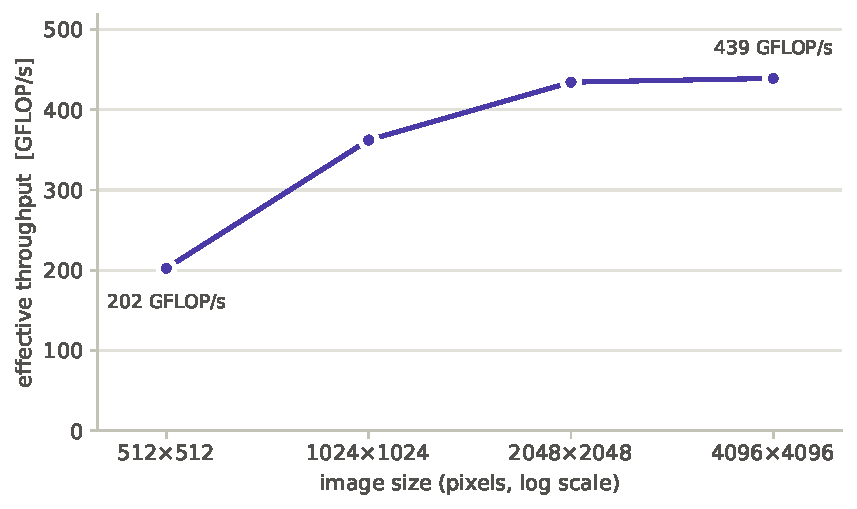
\includegraphics[width=0.85\textwidth]{Immagini/grafici/cuda_saturation}
    \caption{Throughput effettivo della GPU in funzione della dimensione
    dell'immagine (Sweep~B1: blocco $256{\times}1$, $N_{\max}=1000$, job $34424$).
    Il throughput si stabilizza da $2048^2$; il seriale, a circa
    $2{,}88$~GFLOP/s, non è rappresentabile sulla stessa scala.}
    \label{fig:cuda-saturation}
\end{figure}

Dei tre fattori attesi, il trasferimento si può escludere: pesa fra il $3{,}5$ e
il $4{,}6\%$ del tempo a ogni taglia, e non può spiegare un throughput dimezzato.
Anche un costo fisso di lancio spiega poco. I tempi delle due taglie maggiori
crescono in proporzione ai pixel, e la loro retta attribuisce al costo
indipendente dalla taglia circa $0{,}3$~ms; a $512^2$, però, il tempo misurato
supera quella previsione del $77\%$, e a $1024^2$ del $15\%$. La penalità delle
taglie piccole è quindi compatibile con il terzo fattore, il sottoutilizzo della
scheda: con pochi pixel non ci sono abbastanza warp da tenere occupati tutti gli
SM. Senza performance counter non è possibile verificarlo direttamente. Il proxy
di divergenza diminuisce con la risoluzione, da $18\,012$ a $3\,154$, perché pixel
adiacenti diventano più simili; lo Sweep~A ha però mostrato che i cicli sprecati
incidono poco sul tempo, e non possono spiegare la saturazione.

Rispetto al seriale la GPU conviene già alla taglia minima ($S = 70$). Il
confronto con la CPU parallela è disponibile solo a $1024^2$, dove una GPU resta
$4{,}04$ volte più veloce del master--worker MPI su $32$ unità, in accordo con lo
Sweep~A.

\paragraph{Trasferimento (B2) e posizionamento NUMA.}
A risoluzione fissa i byte copiati sono costanti ($16$~MiB), mentre il lavoro
cresce con $N_{\max}$: la frazione del tempo spesa nella copia scende dal
$7{,}1\%$ a $N_{\max}=500$ allo $0{,}8\%$ a $N_{\max}=5000$, come atteso. Un
modello lineare sui tre punti, $T = c + \tau\,\mathcal{W}$, riproduce i tempi
entro $0{,}06$~ms e separa un costo di circa $1{,}5$~ms indipendente da
$N_{\max}$ (copia, allocazione e lancio a questa taglia) da un throughput
marginale di $473$~GFLOP/s, il valore verso cui tende quello effettivo al
crescere del lavoro.

Il log del job documenta il posizionamento: la GPU assegnata ha come core locali
$0$--$31$, cioè il nodo NUMA $0$, mentre il processo è stato eseguito sul core
$42$, sul socket $1$. È il caso cross-NUMA descritto nella
sezione~\ref{sec:cuda-metriche}: ogni copia attraversa anche l'interconnessione
fra i socket. La banda effettiva cresce con la dimensione della copia
(figura~\ref{fig:cuda-copy}), da
$11{,}7$~GB/s per $1$~MiB a $23{,}7$~GB/s per $64$~MiB. Interpolando il tempo di
copia in funzione dei byte si ottengono una banda di circa $24$~GB/s e un costo
fisso di circa $0{,}07$~ms per copia, che penalizza le copie piccole. La banda
asintotica è quindi circa il $77\%$ dei $31{,}5$~GB/s nominali del PCIe~4.0~x16.
A parità di byte la banda oscilla fra $19{,}2$ e $23{,}0$~GB/s nelle tre
esecuzioni a $2048^2$: la singola copia è soggetta a una variabilità non
trascurabile.
\begin{figure}[htbp]
    \centering
    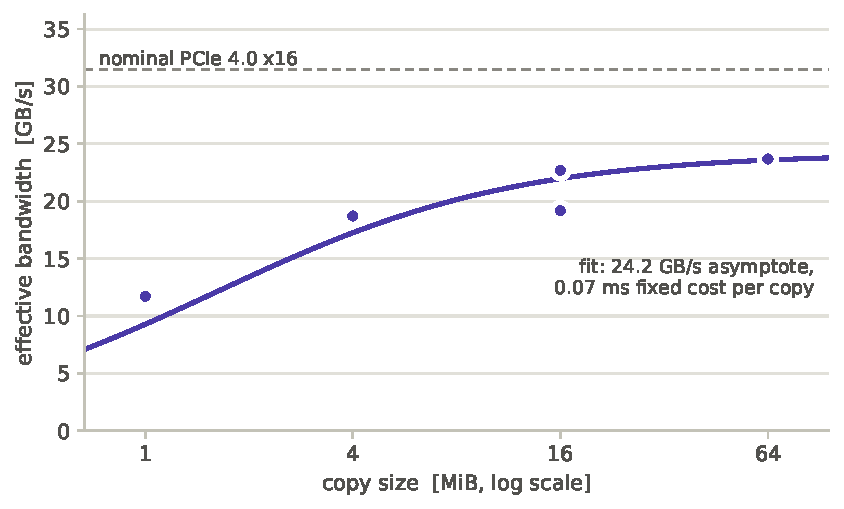
\includegraphics[width=0.85\textwidth]{Immagini/grafici/cuda_copy_bandwidth}
    \caption{Banda effettiva della copia device$\to$host in funzione della
    dimensione della copia, per le sei configurazioni dello Sweep~B (job $34424$,
    processo e GPU su socket diversi). La curva è il modello lineare del tempo di
    copia, con banda asintotica di $24{,}2$~GB/s e costo fisso di $0{,}07$~ms per
    copia; la linea tratteggiata è la banda nominale del PCIe~4.0~x16.}
    \label{fig:cuda-copy}
\end{figure}

Quanto della riduzione rispetto al nominale sia dovuto al passaggio fra i socket
non si può stabilire con un solo job. Il tempo misurato somma i tre contributi, e
separarli richiederebbe un confronto con il caso locale, che SLURM non permette di
scegliere; il valore nominale, inoltre, si riferisce al solo collegamento e non
comprende l'overhead di protocollo. Lo Sweep~A, eseguito senza il log NUMA, ha
copiato $4$~MiB in $0{,}217$~ms contro i $0{,}224$~ms di questo job: un valore
compatibile, che non permette però di attribuirgli un posizionamento.

\paragraph{Sintesi.}
Lo studio della GPU si chiude su tre risultati. La forma del blocco è una leva di
second'ordine, e le grandezze calcolabili dalla matrice degli escape time, pur
esatte, non governano il tempo. La scheda si satura da circa quattro milioni di
pixel, dove raggiunge $439$~GFLOP/s e uno speedup di $152$ rispetto a un core;
sotto quella taglia il calo non dipende dal trasferimento ed è compatibile con il
sottoutilizzo della scheda. Il trasferimento, infine, è un costo marginale che si ammortizza
con il lavoro, ma la sua banda dipende da un posizionamento che SLURM non
garantisce: nel job misurato la copia attraversava i due socket e raggiungeva
circa tre quarti della banda nominale.

